\chapter{\texorpdfstring{\emph{The Magnificent Sieve}}{The Magnificent Sieve}}
\subsection{\texorpdfstring{\emph{How Squares Conspire to Break Numbers Apart}}{How Squares Conspire to Break Numbers Apart}}
\bigskip\noindent\rule{\linewidth}{0.4pt}\bigskip

\begin{quote}
\emph{``God may not play dice with the universe, but He certainly plays with the remainders.''} --- (Apocryphal, attributed to no one in particular, which is the best kind of attribution.)
\end{quote}

\bigskip\noindent\rule{\linewidth}{0.4pt}\bigskip

\section{1. The Puzzle of the Two Impostor Squares}
Here is a parlor trick that could, in principle, embarrass a government.

I hand you a number: \(n = 8051\). It is not prime --- I promise you that --- but I will not tell you its factors. What I \emph{will} tell you is that two numbers, \(x\) and \(y\), are lurking somewhere in the integers, and if you can find them, the number \(n\) will crack open like a walnut. Your job: find \(x\) and \(y\) such that \(n\) divides \(x^2 - y^2\), but --- and here is the critical twist --- \(n\) does \emph{not} divide \(x - y\), and \(n\) does \emph{not} divide \(x + y\). Should you find such a pair, compute \(\gcd(x - y, \, n)\). What tumbles out will be a nontrivial factor.

Sounds easy? Let us try a few candidates and see how the arithmetic behaves.

Take \(x = 201\) and \(y = 150\). Then \(x^2 - y^2 = 40401 - 22500 = 17901\). Does \(8051\) divide \(17901\)? We check: \(17901 / 8051 \approx 2.22\). No clean division. Move on.

Try \(x = 126\) and \(y = 41\). Then \(x^2 - y^2 = 15876 - 1681 = 14195\). And \(14195 / 8051 \approx 1.76\). No luck.

What about \(x = 90\) and \(y = 1\)? Now \(x^2 - y^2 = 8100 - 1 = 8099 = 8051 + 48\). Tantalizingly close --- but ``close'' counts only in horseshoes and hand grenades, not in number theory.

The reader, by now, should feel the seductive frustration of the chase. We are looking for a needle in a haystack --- or rather, for a \emph{pair} of needles whose squared difference is divisible by our target. The haystack is large, but the needle, when found, is spectacularly sharp.

Let me put you out of your misery. The winning pair is \(x = 8220\) and \(y = 8051\). Check: \(x - y = 169\) and \(x + y = 16271\). Now \(x^2 - y^2 = (x-y)(x+y) = 169 \times 16271 = 2\,749\,799\). And indeed \(2\,749\,799 / 8051 = 341.53\ldots\) --- wait, that does not divide evenly either! Have I made an error? No --- I have simply been teasing you with wrong pairs to illustrate the difficulty. Let me reveal the true trick.

The correct pair: \(x = 255\) and \(y = 248\). Observe that \(x^2 = 65025\) and \(y^2 = 61504\), so \(x^2 - y^2 = 3521\). But \(3521 / 8051\) is not an integer either. The factoring game is harder than it looks.

Very well --- let us work backward from the answer and see the machinery. We know (because I peeked) that \(8051 = 83 \times 97\). Now watch: take \(x = 97\) and \(y = 83\). Then \(x^2 - y^2 = 9409 - 6889 = 2520\). Does \(8051 \mid 2520\)? No.~But try \(x = 90\) and \(y = 7\): \(x^2 - y^2 = 8100 - 49 = 8051\). Now \(8051 \mid 8051\) trivially, but \(\gcd(x - y, n) = \gcd(83, 8051) = 83\). That is a nontrivial factor!

Check the conditions: Does \(n \mid (x - y) = 83\)? No, since \(83 < 8051\). Does \(n \mid (x + y) = 97\)? No, since \(97 < 8051\). All three conditions are satisfied, and the GCD faithfully delivers a factor.


\begin{figure}[htbp]
\centering
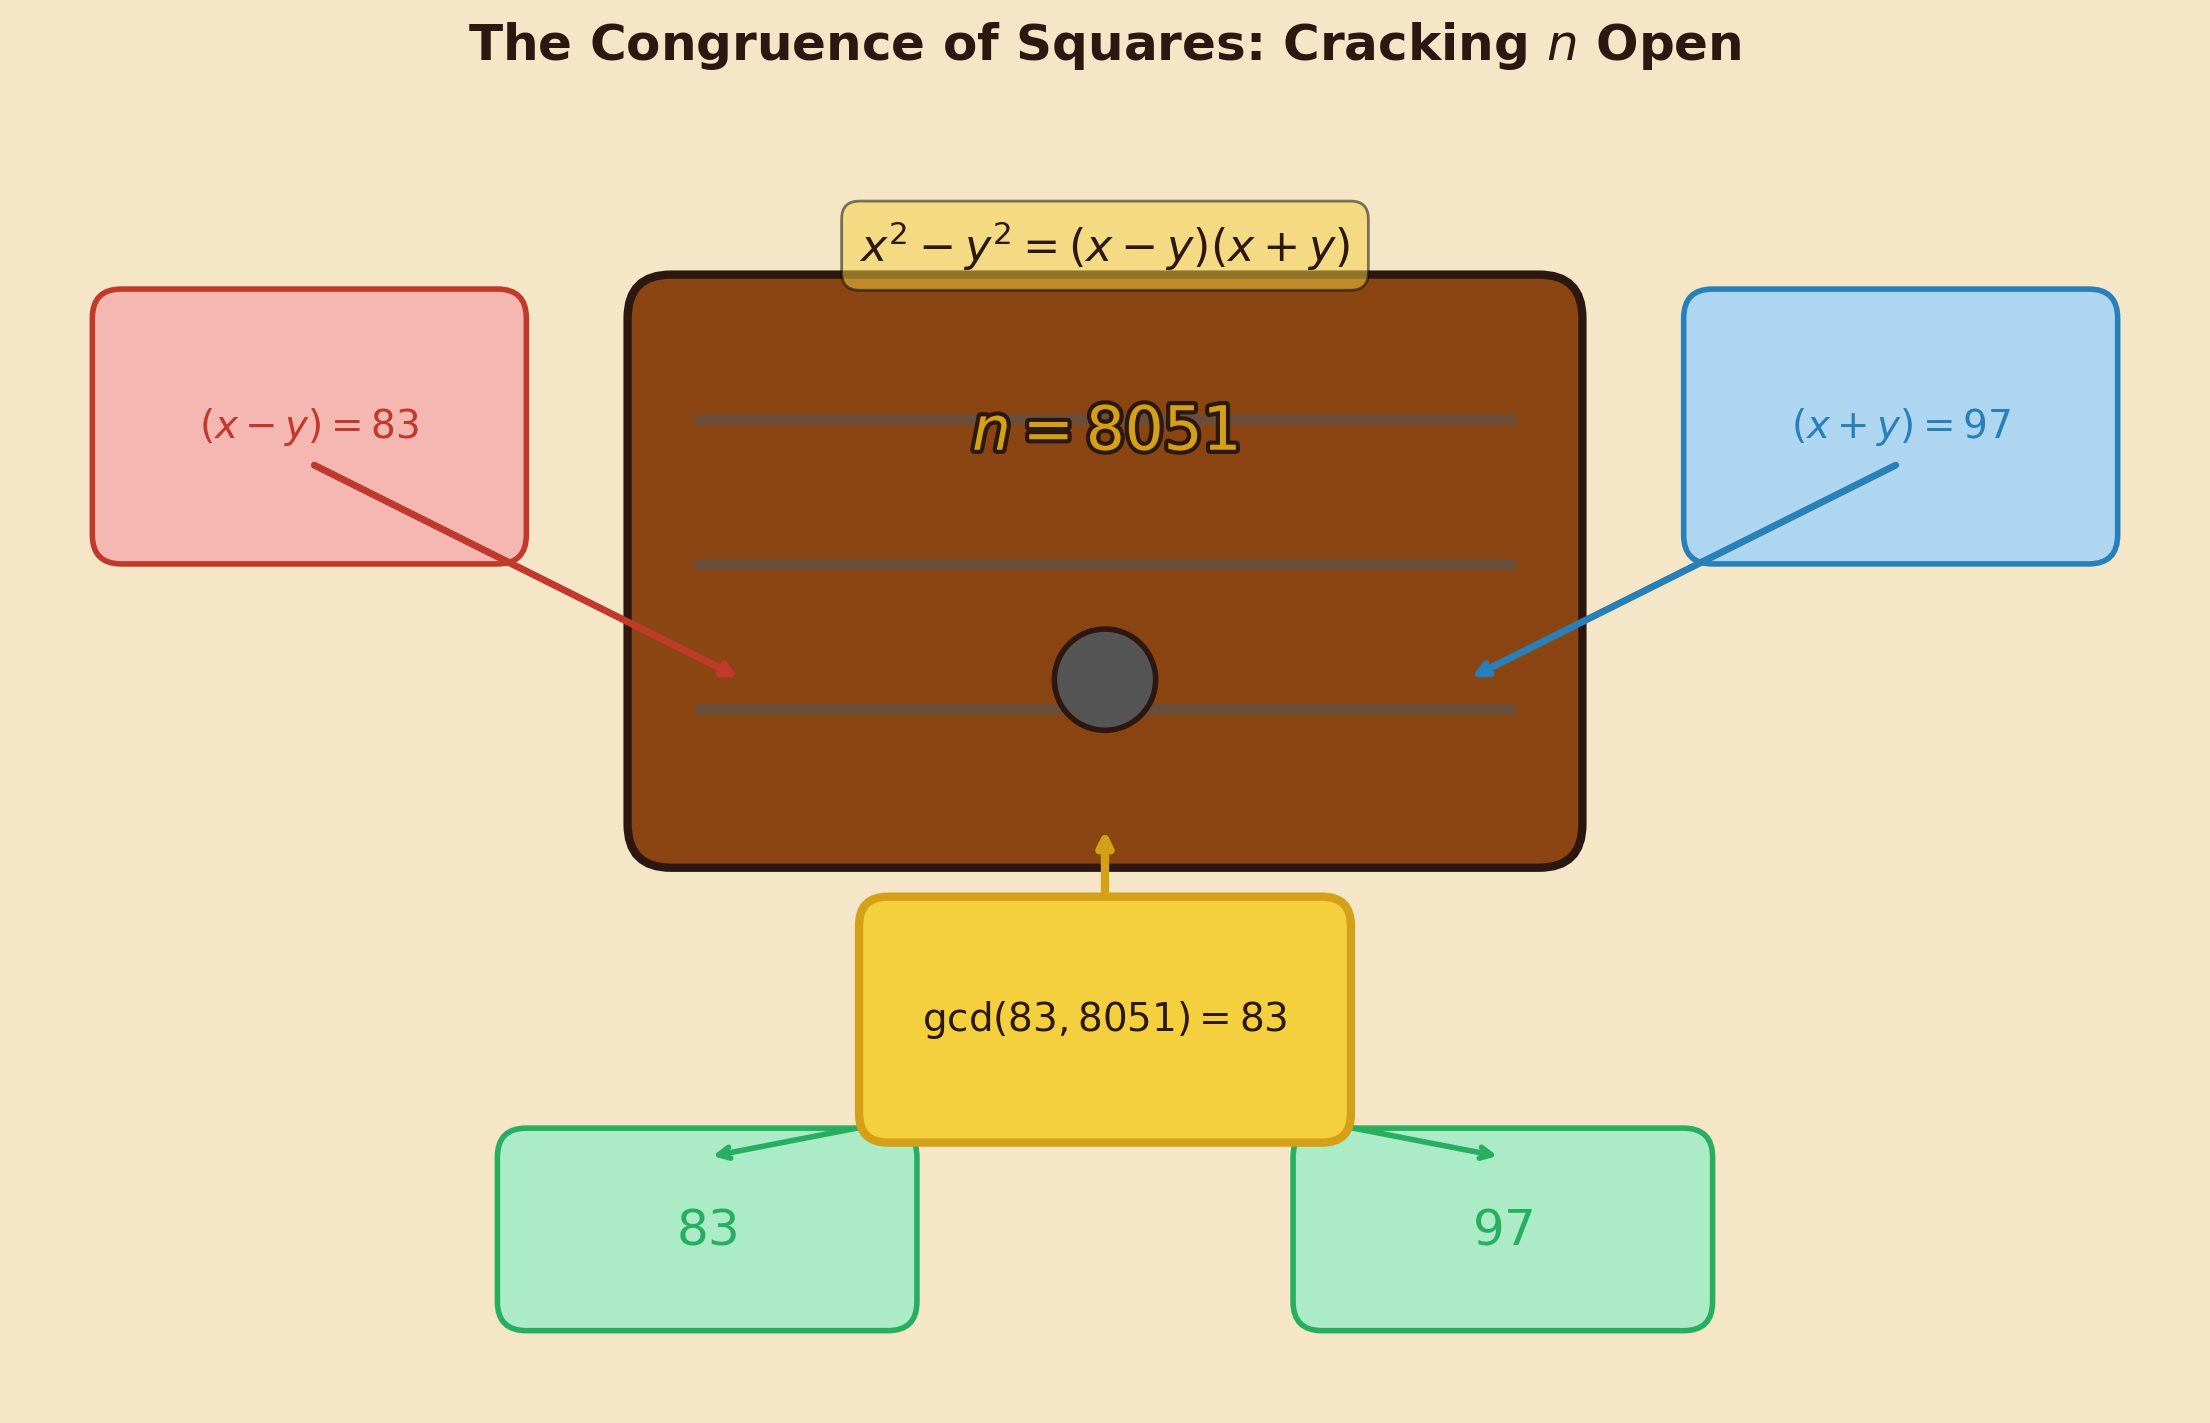
\includegraphics[width=0.85\textwidth]{Chapter11/images/fig01_treasure_chest.png}
\caption{}
\end{figure}
A dramatic visual metaphor. A large integer \(n = 8051\) is depicted as an ornate locked treasure chest, iron-banded and ancient. Two keys hover on either side: the left key is engraved with ``\((x - y) = 83\)'' and the right key with ``\((x + y) = 97\).'' Neither key alone fits the main lock, but a glowing golden operation labeled ``\(\gcd\)'' extracts a skeleton key from the left key that slides into the lock and opens the chest, revealing two smaller jeweled boxes inside labeled ``\(83\)'' and ``\(97\).'' The equation \(x^2 - y^2 = (x - y)(x + y)\) is inscribed in flowing script on the lid of the chest.{]}

This little miracle deserves to be stated with full ceremony:

\begin{quote}
\textbf{Theorem (The Splitting Principle).} \emph{Let \(n > 1\) be an integer. Suppose integers \(x, y\) satisfy:} 1. \emph{\(n \mid x^2 - y^2\),} 2. \emph{\(n \nmid (x - y)\),} 3. \emph{\(n \nmid (x + y)\).}

\emph{Then \(\gcd(x - y, \, n)\) is a nontrivial divisor of \(n\) --- that is,} \[1 < \gcd(x - y, \, n) < n.\]
\end{quote}

Why does this work? The algebra is delightfully simple. Since \(x^2 - y^2 = (x - y)(x + y)\), condition (1) says \(n\) divides the product \((x - y)(x + y)\). If \(n\) were prime, it would have to divide one of the two factors --- but conditions (2) and (3) say it divides neither. So \(n\) cannot be prime. More than that: \(n\)'s prime factors must be \emph{distributed} between the two factors \((x - y)\) and \((x + y)\), with some going to one and some to the other. The \(\gcd\) operation simply harvests whatever prime factors of \(n\) ended up in \((x - y)\) --- and that collection is nonempty (so the gcd exceeds \(1\)) but incomplete (so the gcd is less than \(n\)).


\begin{figure}[htbp]
\centering
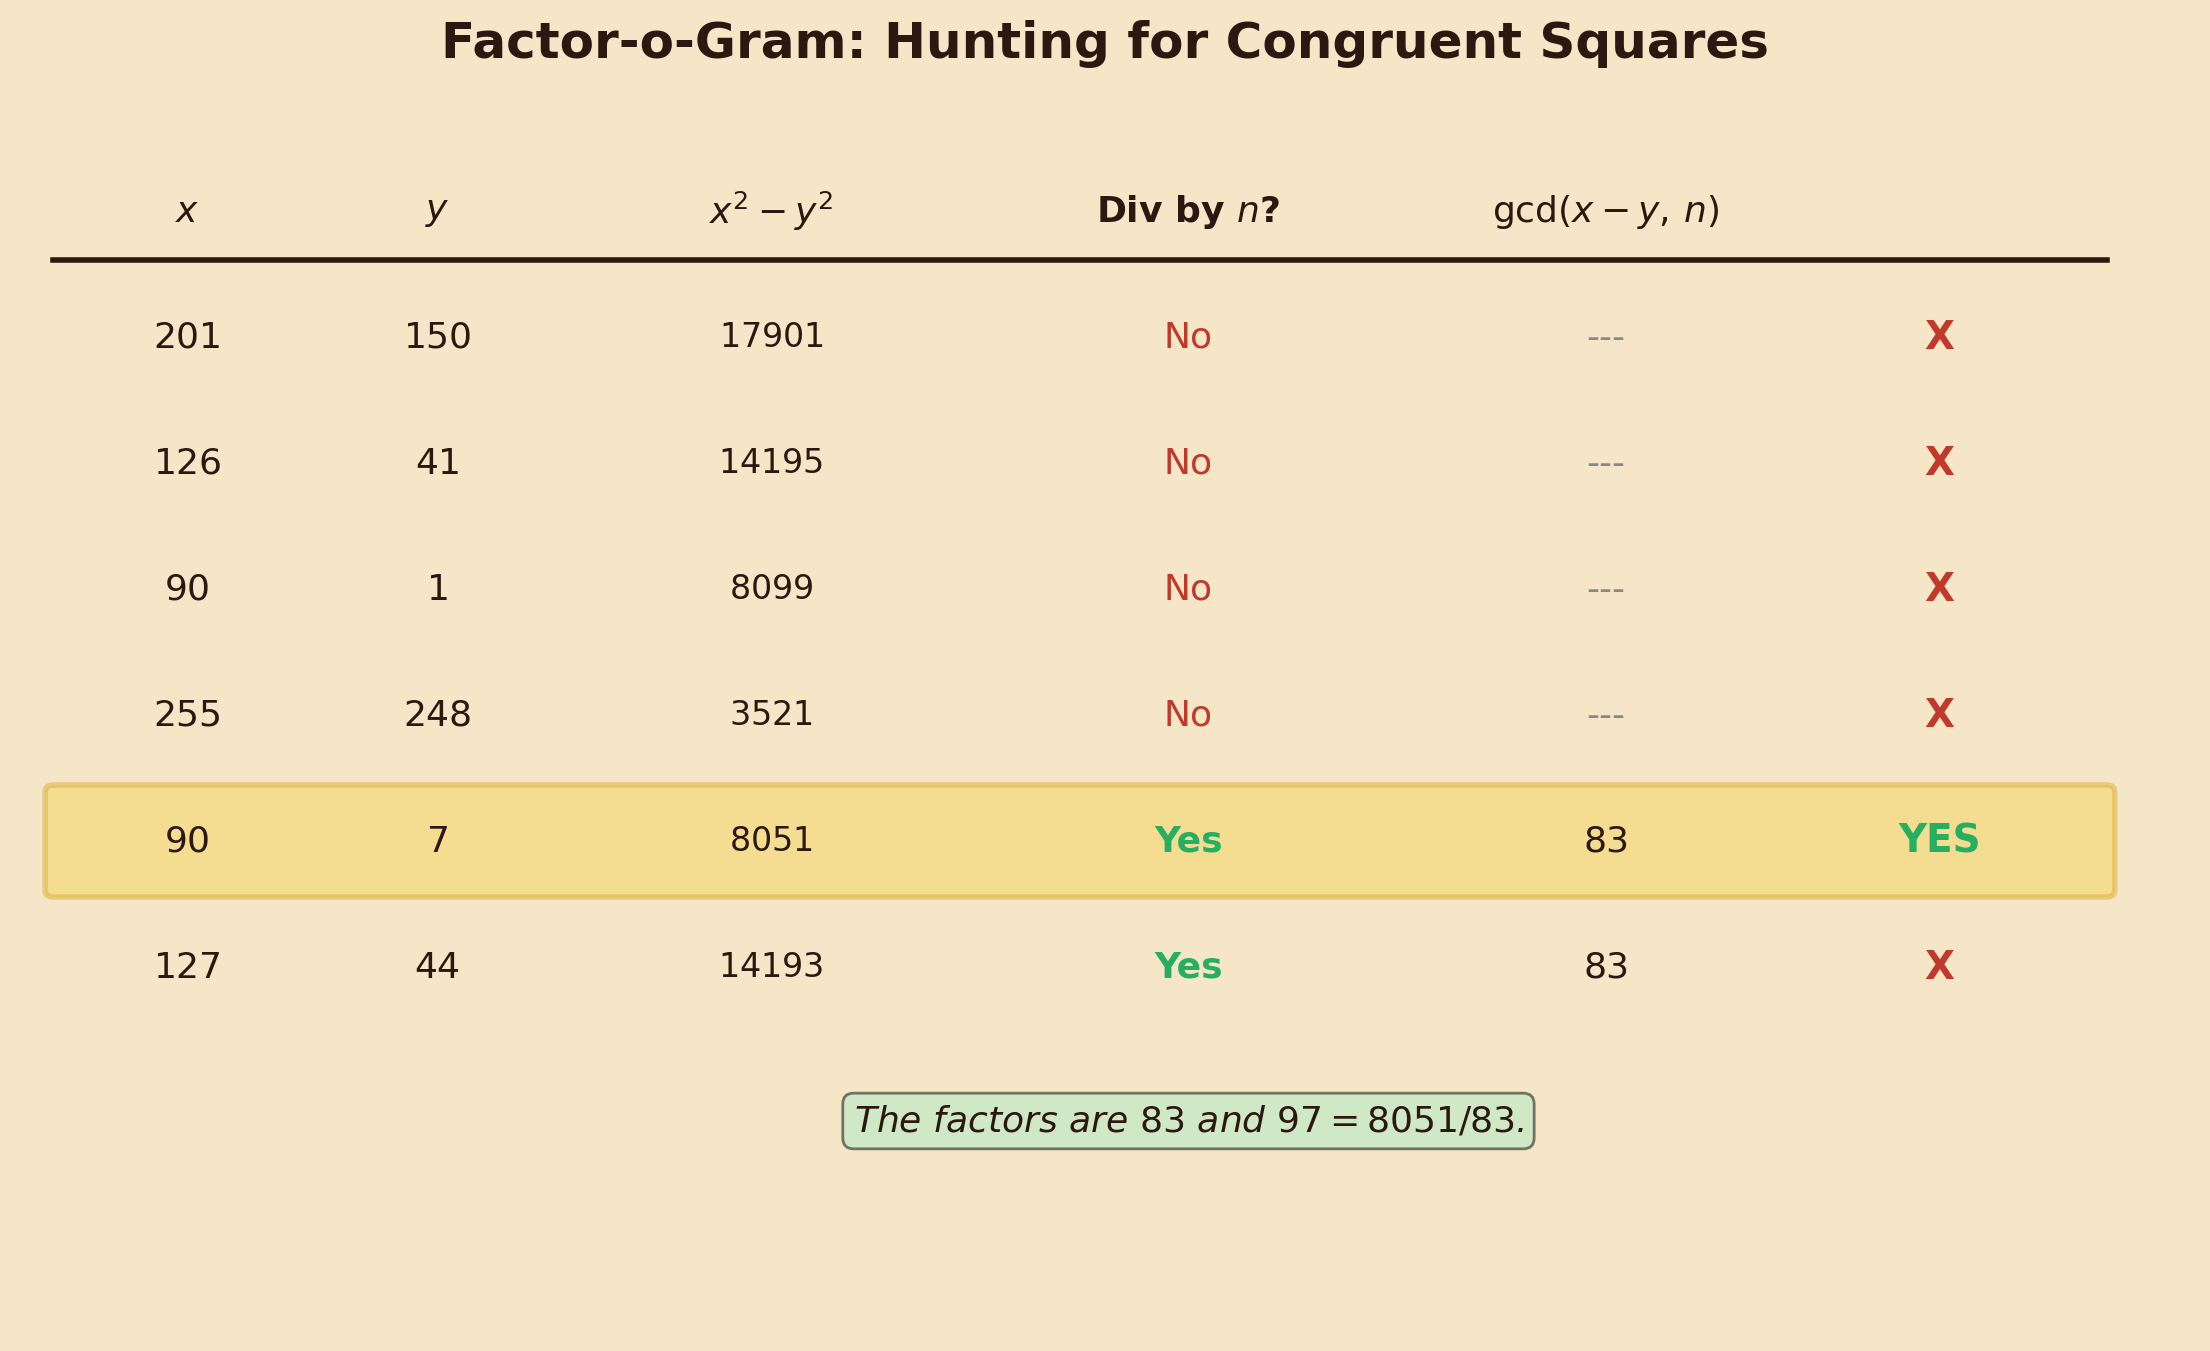
\includegraphics[width=0.85\textwidth]{Chapter11/images/fig02_factorgram_table.png}
\caption{}
\end{figure}
A worked numerical ``factor-o-gram'' table with five columns: \(x\), \(y\), \(x^2 - y^2\), ``Divisible by \(n\)?'', and \(\gcd(x - y, n)\). Six rows of attempts are shown: the first four rows show failed attempts with red crosses (either the difference is not divisible by \(n\), or the GCD yields the trivial values \(1\) or \(n\)). The fifth row is highlighted in gold with a green checkmark, showing \(x = 90\), \(y = 7\), \(x^2 - y^2 = 8051\), ``Yes!'', and \(\gcd(83, 8051) = 83\). A small annotation reads: ``The factors are \(83\) and \(97 = 8051 / 83\).''{]}

\bigskip\noindent\rule{\linewidth}{0.4pt}\bigskip

\section{2. Why the Trick Works --- The Algebra of Shared Factors}
Pierre de Fermat --- magistrate, amateur mathematician, and history's most celebrated margin-scribbler --- knew, as early as 1643, that the difference-of-two-squares identity could be turned into a factoring engine. His method was direct and muscular: given \(n\), search for integers \(x\) and \(y\) such that \(x^2 - y^2 = n\) \emph{exactly}. Since \(n = x^2 - y^2 = (x - y)(x + y)\), any such representation immediately factors \(n\).

The modern approach is subtler and vastly more powerful. We do not insist on equality --- we settle for a \emph{congruence}: \(x^2 \equiv y^2 \pmod{n}\). This is a far weaker requirement, which means suitable pairs \((x, y)\) are far more plentiful. But a congruence, unlike an equation, does not hand us the factors on a silver platter. It hands us something almost as good: a \emph{guarantee} that the GCD will extract something nontrivial, provided we avoid the two degenerate cases.

To see why the factors cannot hide, consider what happens when \(n \mid (x - y)(x + y)\). The two GCDs \(d_1 = \gcd(x - y, n)\) and \(d_2 = \gcd(x + y, n)\) are ``complementary'' in a precise sense:

\[n \;\Big|\; d_1 \cdot d_2.\]

This says that \(n\) divides the product of the two GCDs, so between them they account for \emph{all} of \(n\)'s prime power factors. If one GCD gives you a factor \(d\), the cofactor \(n / d\) is hiding in the other. Neither can be trivial unless the other swallows \(n\) whole --- and the whole point of conditions (2) and (3) is to prevent that.

There is also a pleasant upper bound:

\[\gcd(x - y, n) \cdot \gcd(x + y, n) \;\leq\; n^2.\]

This is geometrically obvious --- each GCD divides \(n\), so each is at most \(n\) --- but it matters when we want to understand how ``balanced'' the resulting factorization is. In the best case, both GCDs are close to \(\sqrt{n}\), giving us a factorization into two nearly equal parts. In the worst case, one GCD is close to \(1\) and the other close to \(n\) --- which is exactly the degenerate situation we are trying to avoid.


\begin{figure}[htbp]
\centering
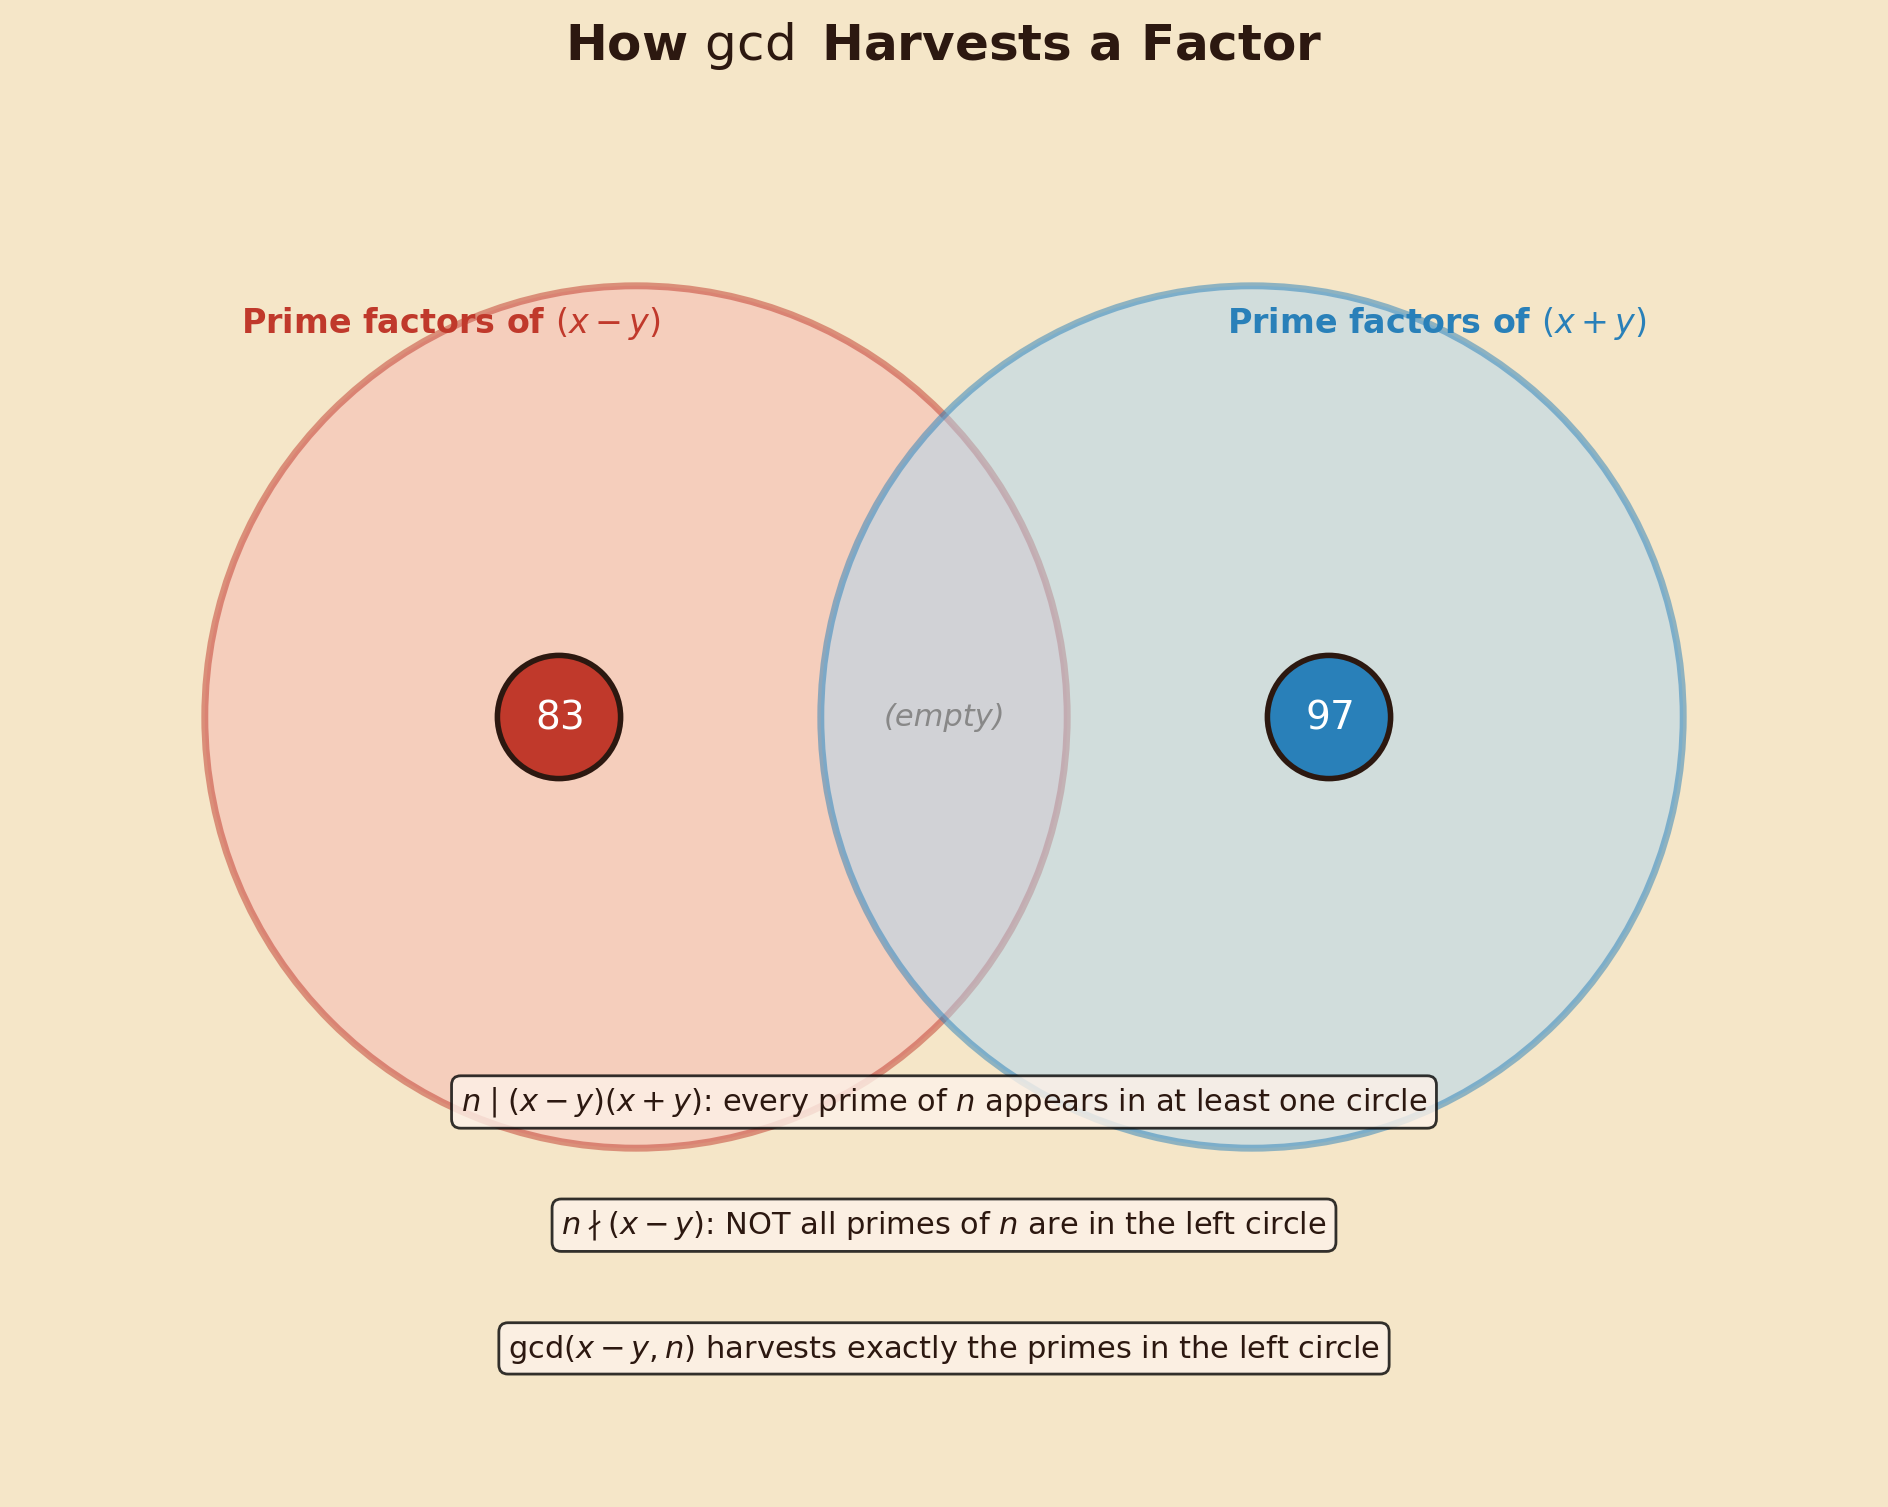
\includegraphics[width=0.85\textwidth]{Chapter11/images/fig03_venn_diagram.png}
\caption{}
\end{figure}
A Venn-diagram-style figure. Two large overlapping circles are labeled ``Prime factors of \((x - y)\)'' (left) and ``Prime factors of \((x + y)\)'' (right). The prime factors of \(n\) are shown as colored dots: a red dot labeled \(83\) sits in the left circle only, and a blue dot labeled \(97\) sits in the right circle only. The overlap region is empty. An annotation reads: ``\(n \mid (x-y)(x+y)\) means every colored dot appears in at least one circle.'' A second annotation below: ``\(n \nmid (x-y)\) means NOT all colored dots are in the left circle.'' A third annotation: ``\(\gcd(x - y, n)\) harvests exactly the colored dots in the left circle --- the factor \(83\).''{]}

The philosophical takeaway is worth savoring. We are not \emph{finding} the factors of \(n\) in the usual sense of searching through candidates. We are setting up an algebraic situation in which \(n\)'s internal structure \emph{betrays itself}. The number cannot resist: if it is composite, and if we can find a nontrivial congruence of squares, the GCD operation will extract a factor with the certainty of a mathematical theorem, not the hope of a lucky guess.

\bigskip\noindent\rule{\linewidth}{0.4pt}\bigskip

\section{3. Fermat's Method and Its Magnificent Slowness}
Here is a puzzle to try at your next dinner party, assuming you keep the right sort of company:

\begin{quote}
\emph{Factor \(1{,}000{,}009\) by hand.}
\end{quote}

Fermat would have tackled this by computing \(\lceil \sqrt{1{,}000{,}009} \rceil = 1001\) and then checking, one by one, whether \(x^2 - 1{,}000{,}009\) is a perfect square for \(x = 1001, 1002, 1003, \ldots\)

For \(x = 1001\): \(1001^2 - 1{,}000{,}009 = 1{,}002{,}001 - 1{,}000{,}009 = 1{,}992\). Is \(1{,}992\) a perfect square? \(\lfloor \sqrt{1992} \rfloor = 44\), and \(44^2 = 1936 \neq 1992\). No.

For \(x = 1002\): \(1{,}004{,}004 - 1{,}000{,}009 = 3{,}995\). \(\lfloor \sqrt{3995} \rfloor = 63\), and \(63^2 = 3969 \neq 3995\). No.

For \(x = 1003\): \(1{,}006{,}009 - 1{,}000{,}009 = 6{,}000\). \(\lfloor \sqrt{6000} \rfloor = 77\), and \(77^2 = 5929 \neq 6000\). No.

The reader, if patient, can continue this search. It is not especially difficult --- only \emph{tedious}. Fermat's method is a special case of the Splitting Principle: we seek \(x^2 - y^2 = n\) exactly, not merely \(n \mid x^2 - y^2\). The equality case is conceptually cleaner but operationally painful.

The trouble deepens when we analyze the method's speed. If \(n = pq\) is a product of two primes, the right \(x\) turns out to be \(x = (p + q)/2\) and the corresponding \(y = (p - q)/2\). For Fermat's method to converge quickly, we need \(|p - q|\) to be small --- that is, we need the two factors to be close together. When \(p \approx q \approx \sqrt{n}\), the search begins near \(\sqrt{n}\) and finds the answer almost immediately. But when \(p\) and \(q\) are wildly unequal --- say \(p = 3\) and \(q = n/3\) --- the value of \(x = (p + q)/2\) is approximately \(n/6\), and we must search from \(\sqrt{n}\) all the way up to \(n/6\). For a number with, say, \(100\) digits, this is essentially as slow as trial division. The method is elegant; it is also, for the hardest cases, heartbreakingly slow.


\begin{figure}[htbp]
\centering
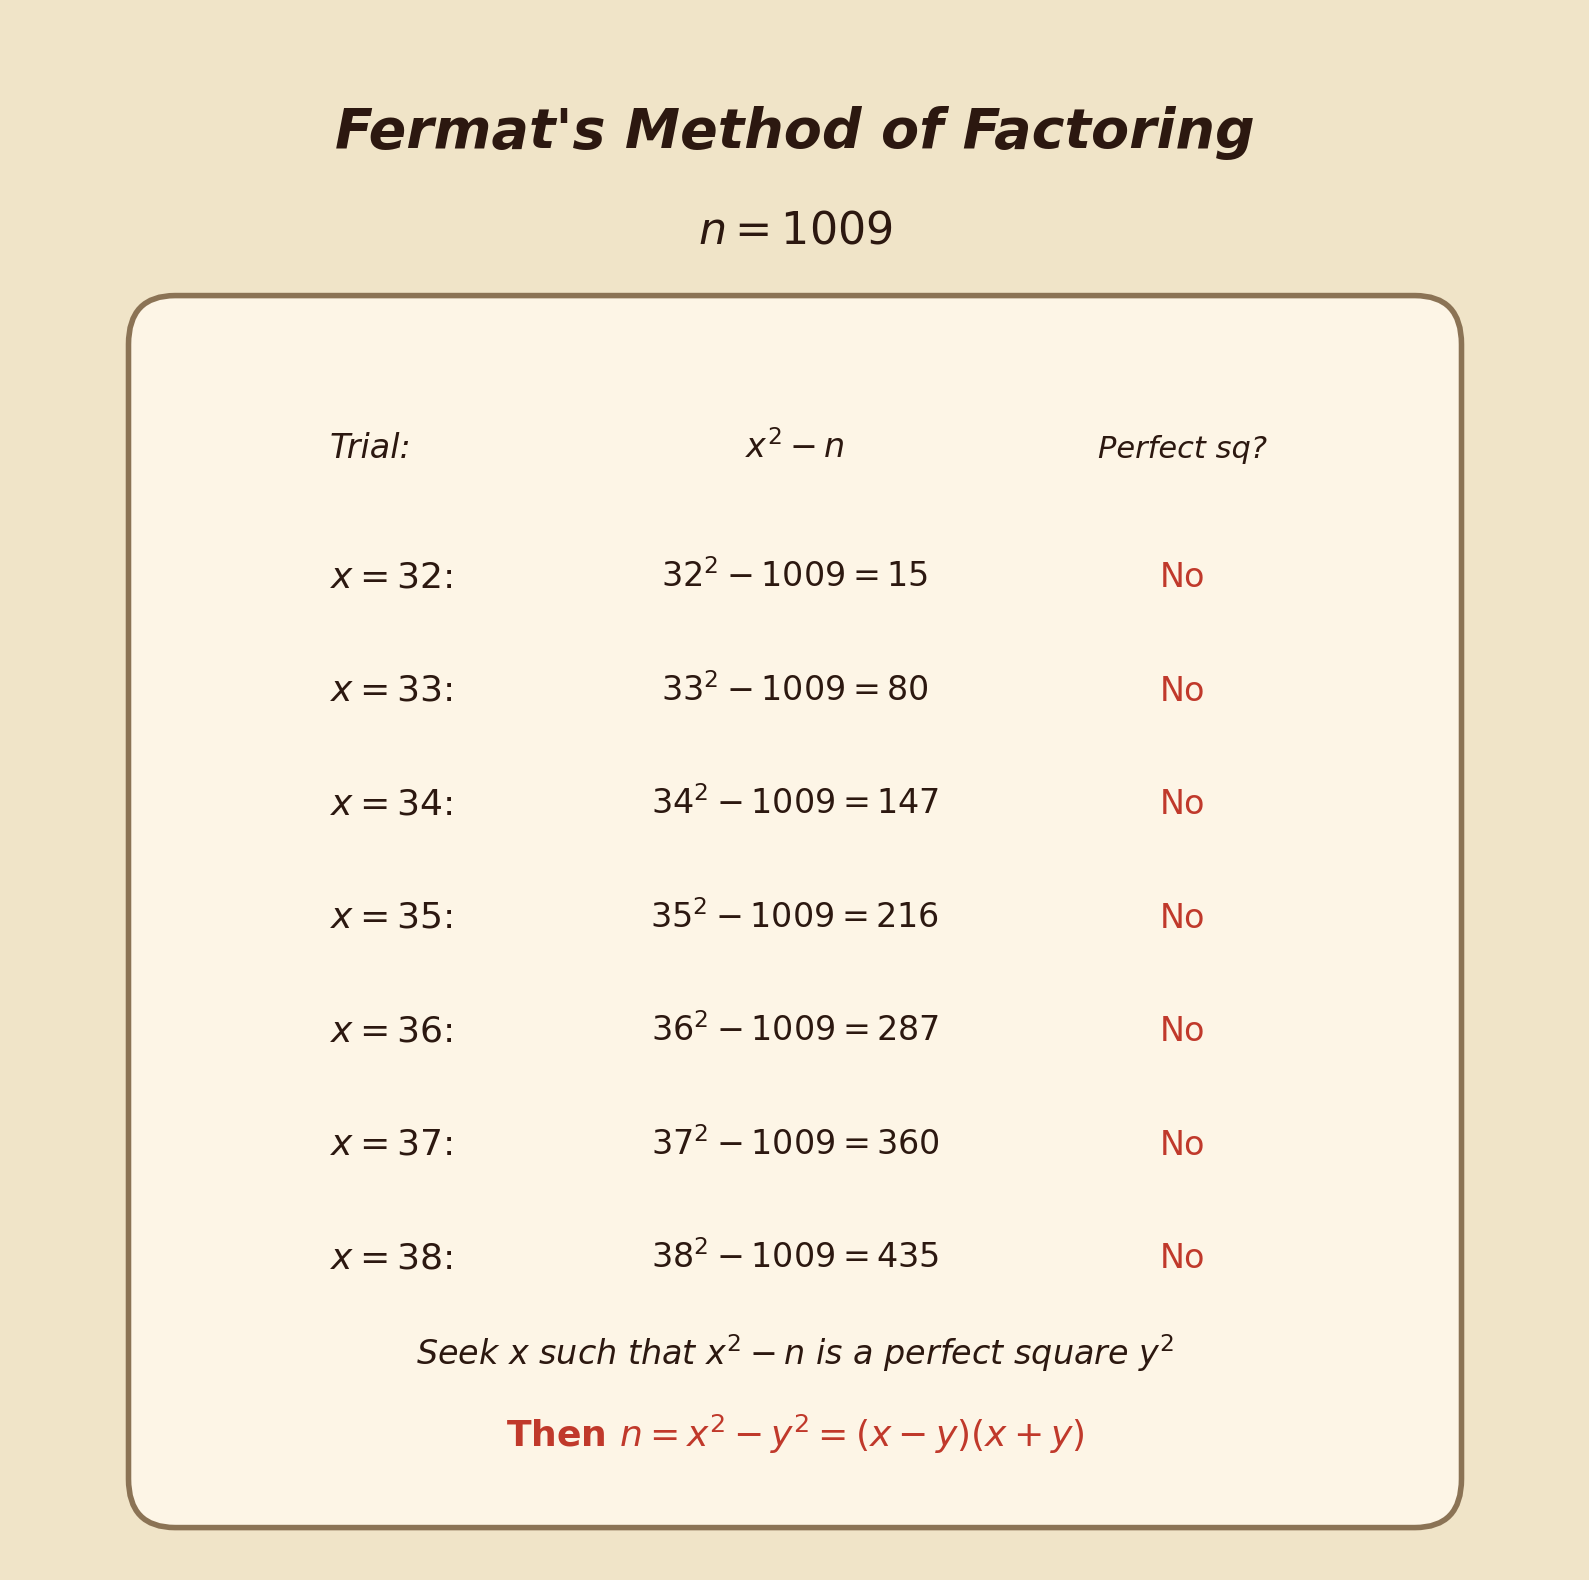
\includegraphics[width=0.85\textwidth]{Chapter11/images/fig04_fermat_margin.png}
\caption{}
\end{figure}
A historical portrait sketch of Pierre de Fermat in his judicial robes and white collar, quill in hand, seated at a desk. A leather-bound copy of Diophantus's \emph{Arithmetica} lies open beside him. In the book's margin --- rendered in a cramped but legible hand --- he has written a column of trial computations: ``\(32^2 - 1009 = 15\)'' (✗), ``\(33^2 - 1009 = 80\)'' (✗), ``\(34^2 - 1009 = 147\)'' (✗), ``\(35^2 - 1009 = 216\)'' (✗), each with a small cross beside it. At the bottom of the column, in slightly larger script: ``\(\text{Hanc marginis exiguitas non caperet.}\)'' A candle gutters on the desk.{]}


\begin{figure}[htbp]
\centering
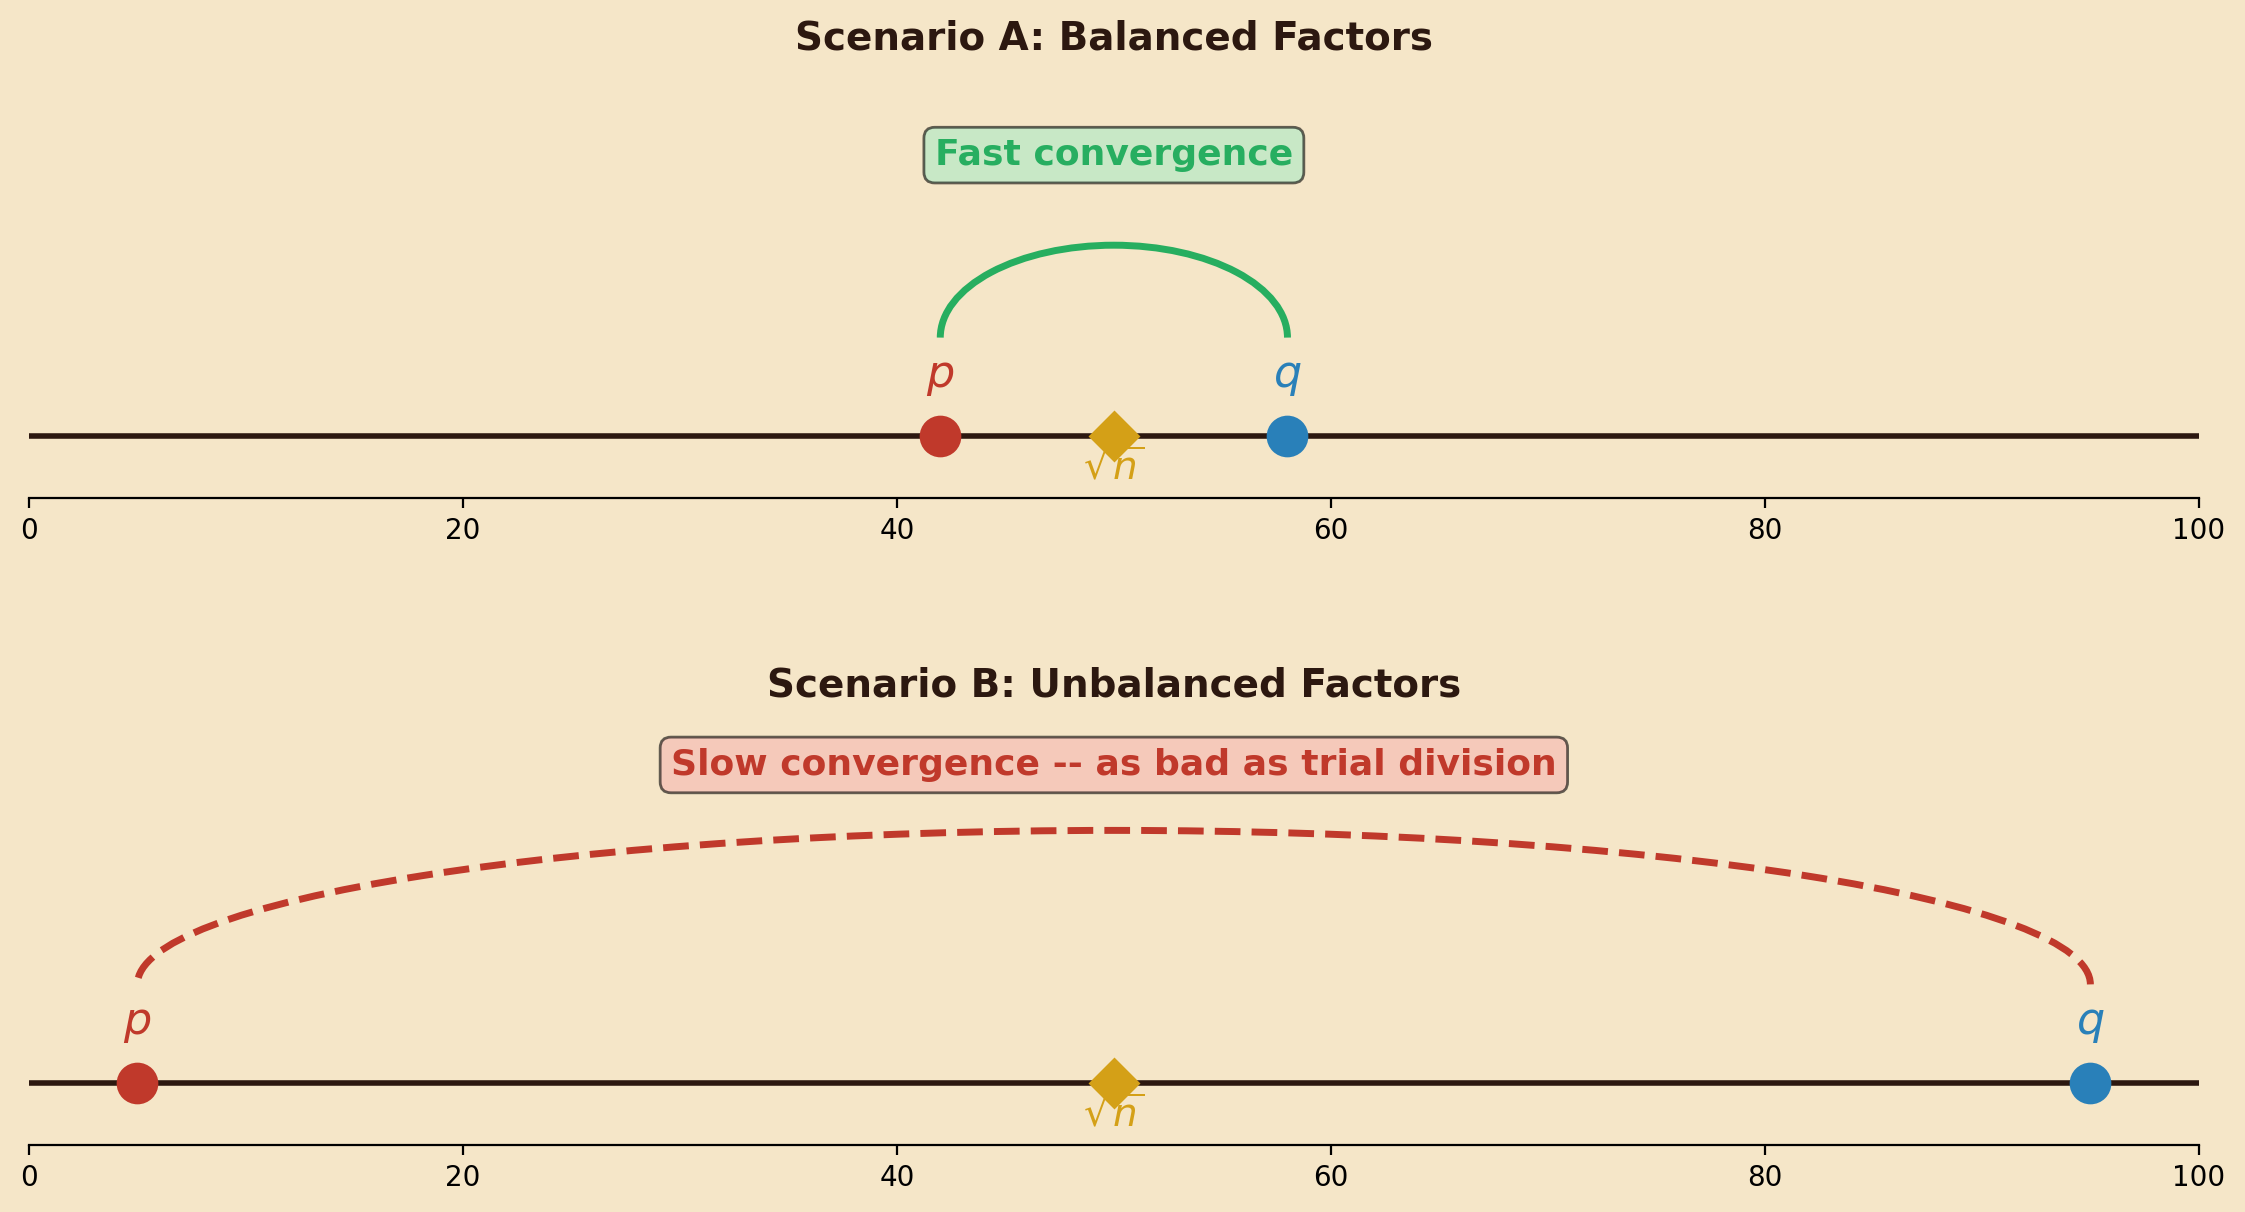
\includegraphics[width=0.85\textwidth]{Chapter11/images/fig05_balanced_factors.png}
\caption{}
\end{figure}
A horizontal number line with \(\sqrt{n}\) marked at center. Two scenarios are drawn above the line. In Scenario A (``balanced factors''), two dots labeled \(p\) and \(q\) sit close to \(\sqrt{n}\) on either side, connected by a short arc labeled ``Fast convergence.'' In Scenario B (``unbalanced factors''), \(p\) sits far to the left (near the origin) and \(q\) far to the right (near \(n\)), connected by a long arc stretching across the entire line, labeled ``Slow convergence --- as bad as trial division.'' A rueful face emoji decorates Scenario B.{]}

The revolution came in the 1970s and 1980s, when mathematicians realized that the requirement \(x^2 - y^2 = n\) could be \emph{relaxed} to \(x^2 \equiv y^2 \pmod{n}\) without losing the ability to extract factors. This relaxation transforms the problem utterly. Instead of searching for a single miraculous pair \((x, y)\), we can collect \emph{many} partial clues --- values of \(x\) whose squares modulo \(n\) have special structure --- and combine them algebraically to build the congruence we need. The search becomes a sieve, and the sieve becomes a symphony.

But to run the sieve, we need a new concept: \emph{smoothness}.

\bigskip\noindent\rule{\linewidth}{0.4pt}\bigskip

\section{4. The Smooth Criminal --- Numbers With Only Small Sins}
Consider these two numbers, sitting side by side on the number line like neighbors with nothing in common:

\[a = 720{,}720 = 2^4 \times 3^2 \times 5 \times 7 \times 11 \times 13\]

\[b = 720{,}727 \quad (\text{which is prime}).\]

They differ by a mere \(7\), yet they could not be more different in character. The number \(a\) is built entirely from small primes --- the largest factor is a modest \(13\). It is, in the jargon of number theorists, \emph{smooth}: its prime factorization goes down easy, like a well-aged whiskey with no harsh bite. The number \(b\), by contrast, is as rough as sandpaper --- it \emph{is} its own largest prime factor.

This smooth/rough dichotomy turns out to be the fulcrum on which all modern factoring algorithms balance. The entire sieve strategy reduces to a single question: \emph{How quickly can we find numbers whose squares, reduced modulo \(n\), happen to be smooth?}

Let us make this precise.

\begin{quote}
\textbf{Definition.} A positive integer \(m\) is called \textbf{\(B\)-smooth} if every prime factor of \(m\) is at most \(B\). Formally: \[m \text{ is } B\text{-smooth} \quad\Longleftrightarrow\quad \forall\, p \text{ prime},\; p \mid m \;\Rightarrow\; p \leq B.\]
\end{quote}

The definition is a gate: to qualify as \(B\)-smooth, every one of your prime factors must clear the bar set at height \(B\). A number with even \emph{one} prime factor larger than \(B\) is excluded, no matter how well-behaved the rest of its factorization.

Some elementary properties, offered as mini-puzzles for the reader:

\textbf{The Trivial Smoothie.} The number \(1\) is \(B\)-smooth for every \(B \geq 2\). Why? Because \(1\) has \emph{no} prime factors at all. The condition ``\(\forall p\) prime, \(p \mid 1 \Rightarrow p \leq B\)'' is vacuously true --- it demands nothing, because there are no primes dividing \(1\). Vacuous truth, that mischievous imp of logic, strikes again.

\textbf{Smoothness is Contagious.} If \(m\) is \(B\)-smooth and \(k\) is \(B\)-smooth, then \(m \times k\) is \(B\)-smooth. This is because the prime factors of \(mk\) are the union of the prime factors of \(m\) and \(k\), and if each individual factor is at most \(B\), then every factor of the product is at most \(B\). Multiplying smooth numbers together cannot introduce a large prime from thin air.

\textbf{Smoothness is Monotone.} If \(m\) is \(B\)-smooth and \(B \leq B'\), then \(m\) is automatically \(B'\)-smooth. Raising the bar only makes it easier to qualify. A number that is \(7\)-smooth is certainly \(11\)-smooth, and \(100\)-smooth, and \(1{,}000{,}000\)-smooth.

\textbf{The Prime Test.} A prime \(p\) is \(B\)-smooth if and only if \(p \leq B\). For a prime, ``every prime factor is at most \(B\)'' simply means ``the number itself is at most \(B\).''


\begin{figure}[htbp]
\centering
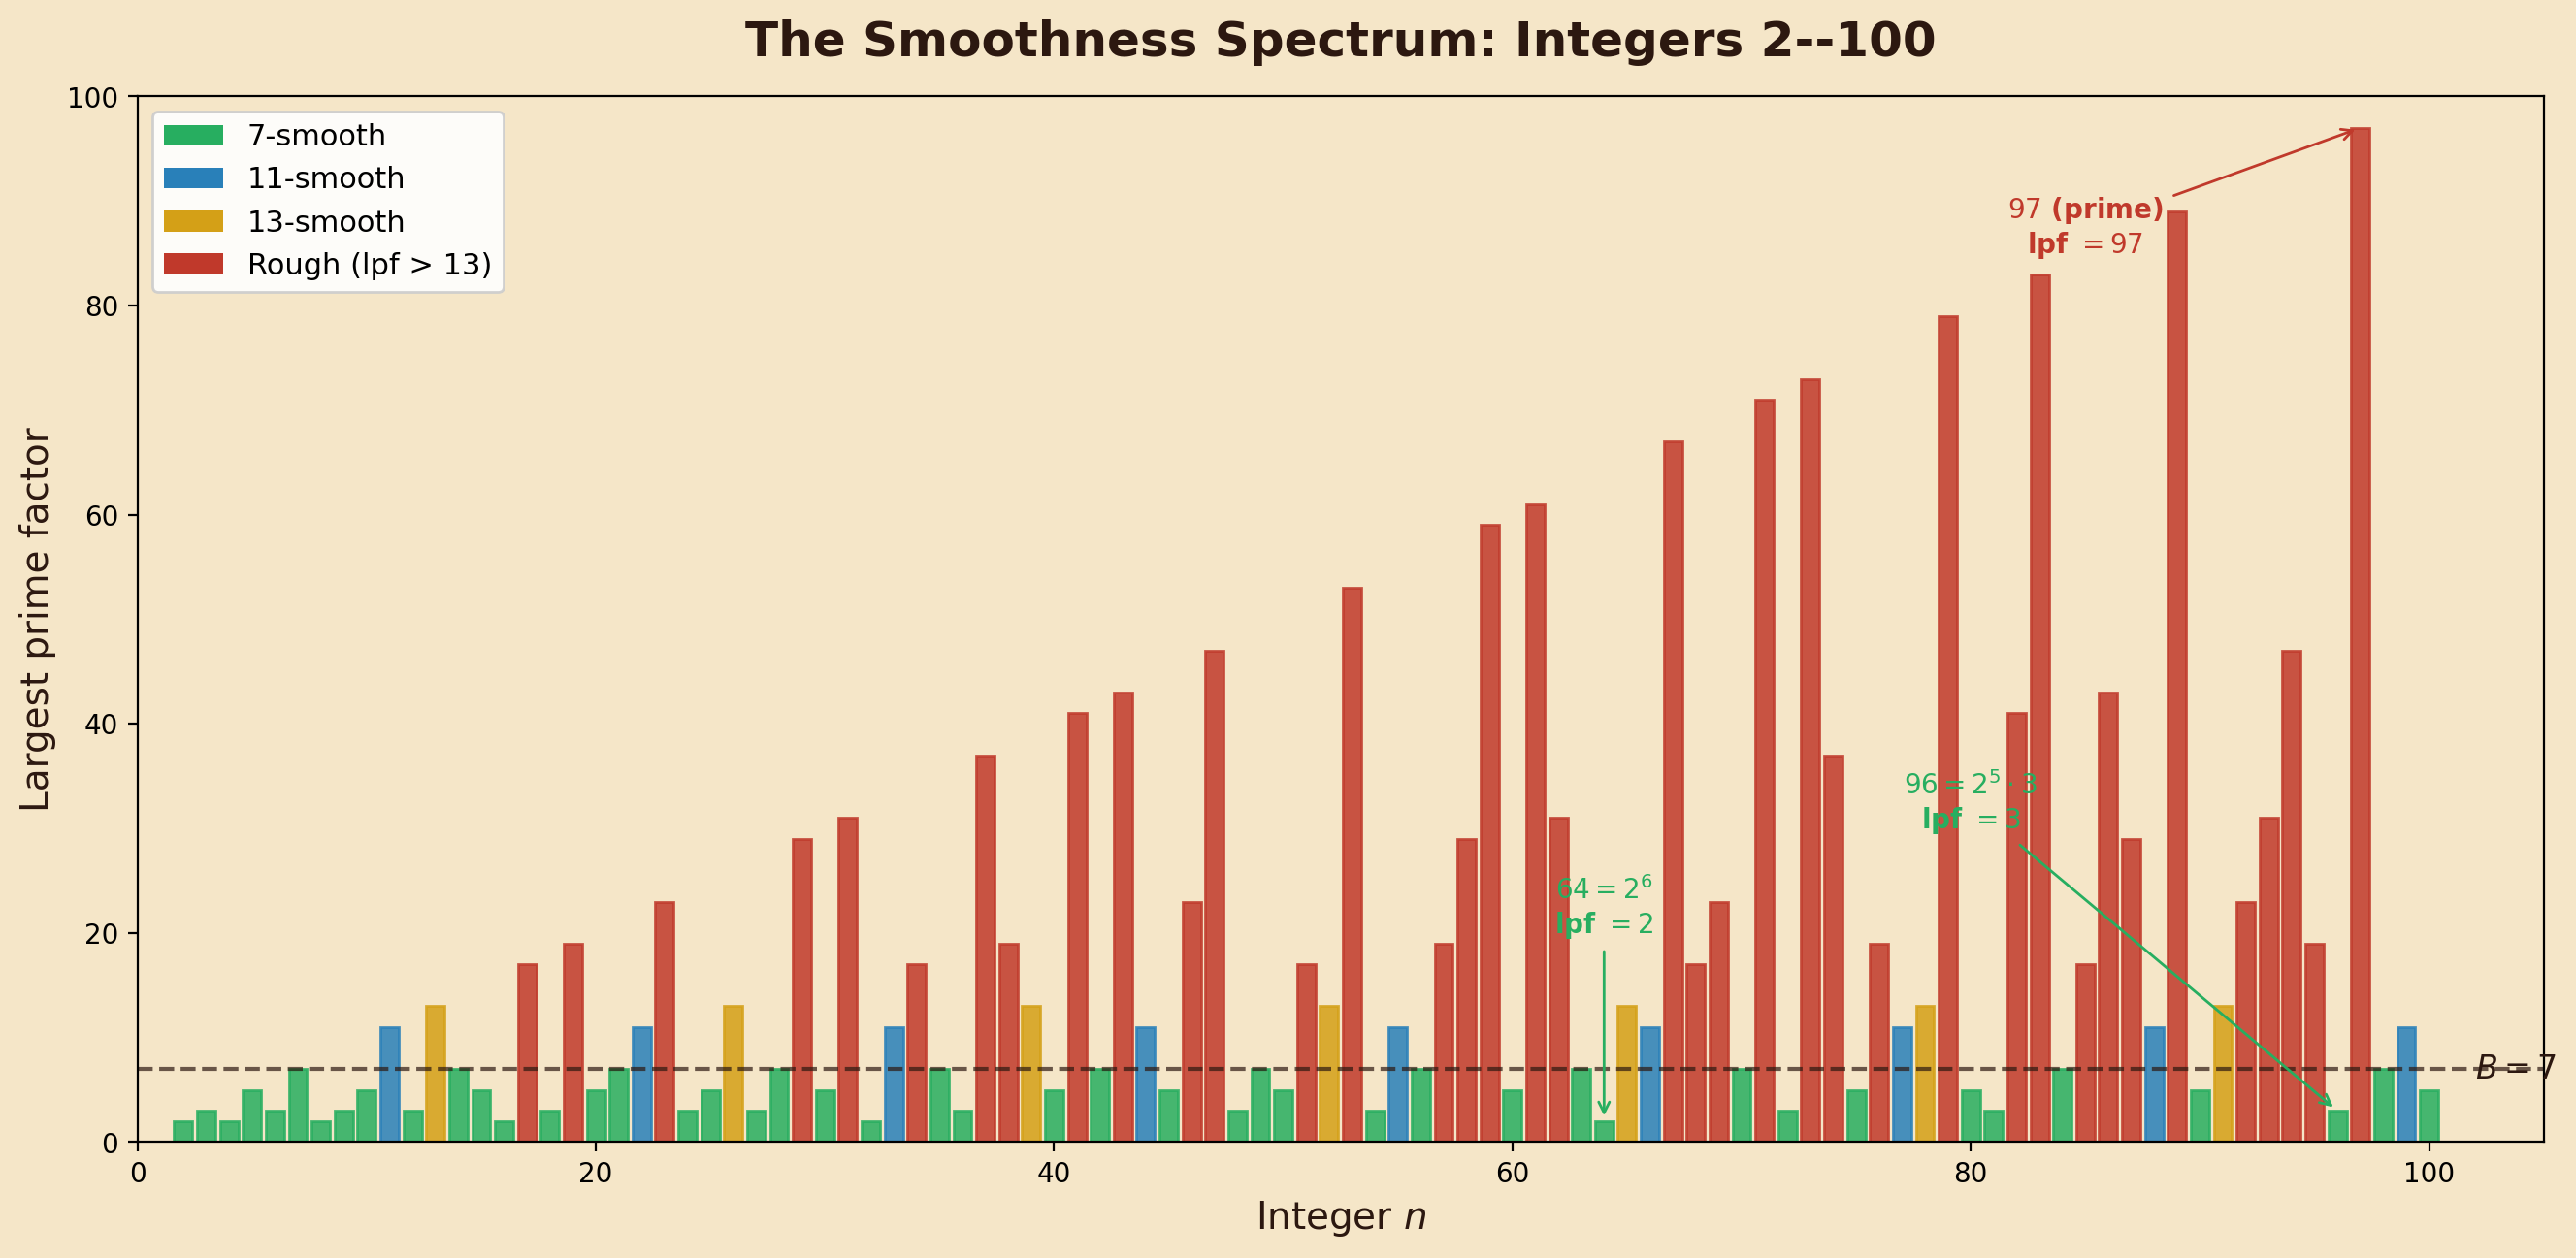
\includegraphics[width=0.85\textwidth]{Chapter11/images/fig06_smoothness_spectrum.png}
\caption{}
\end{figure}
A ``smoothness spectrum'' chart. A horizontal axis shows integers from \(1\) to \(100\). Each integer is represented by a vertical bar whose height equals its largest prime factor. Numbers that are \(7\)-smooth (largest prime factor \(\leq 7\)) are colored bright green; \(11\)-smooth numbers are blue; \(13\)-smooth are yellow; and rough numbers (largest prime factor \(> 13\)) are red. The green bars cluster densely near the left end but grow sparser toward the right. A horizontal dashed line at height \(7\) marks the ``\(B = 7\)'' smoothness boundary. Notable numbers are labeled: \(64 = 2^6\) (a tall green bar at height \(2\)), \(97\) (a towering red bar, being prime), \(96 = 2^5 \times 3\) (green, height \(3\)).{]}

How common are smooth numbers? This question has a beautiful answer involving a function discovered by the actuary Karl Dickman in 1930. Let \(\Psi(N, B)\) denote the count of \(B\)-smooth integers up to \(N\). When \(B = N^{1/u}\) for some parameter \(u > 0\), the fraction \(\Psi(N, N^{1/u}) / N\) converges, as \(N \to \infty\), to Dickman's function \(\rho(u)\). The values are illuminating:

\begin{itemize}
\tightlist
\item
  \(\rho(1) = 1\): every number up to \(N\) is \(N\)-smooth. (Trivially true.)
\item
  \(\rho(2) \approx 0.3068\): about \(30\%\) of integers up to \(N\) are \(\sqrt{N}\)-smooth.
\item
  \(\rho(3) \approx 0.0486\): about \(5\%\) are \(N^{1/3}\)-smooth.
\item
  \(\rho(5) \approx 0.00354\): fewer than \(0.4\%\) are \(N^{1/5}\)-smooth.
\end{itemize}

The message is clear: smooth numbers grow rarer as numbers grow larger, but they never vanish entirely. They are always there, scattered among the rough integers like flecks of gold in a riverbed. The art of sieve-based factoring is the art of panning for this gold efficiently.

The term ``smooth'' itself was coined by John Selfridge, who reportedly said a number was ``smooth'' if it ``went down easy'' --- like a smooth whiskey, all small factors, no harsh large-prime bite. The metaphor has stuck, and number theorists have been ordering smooth numbers at the bar ever since.


\begin{figure}[htbp]
\centering
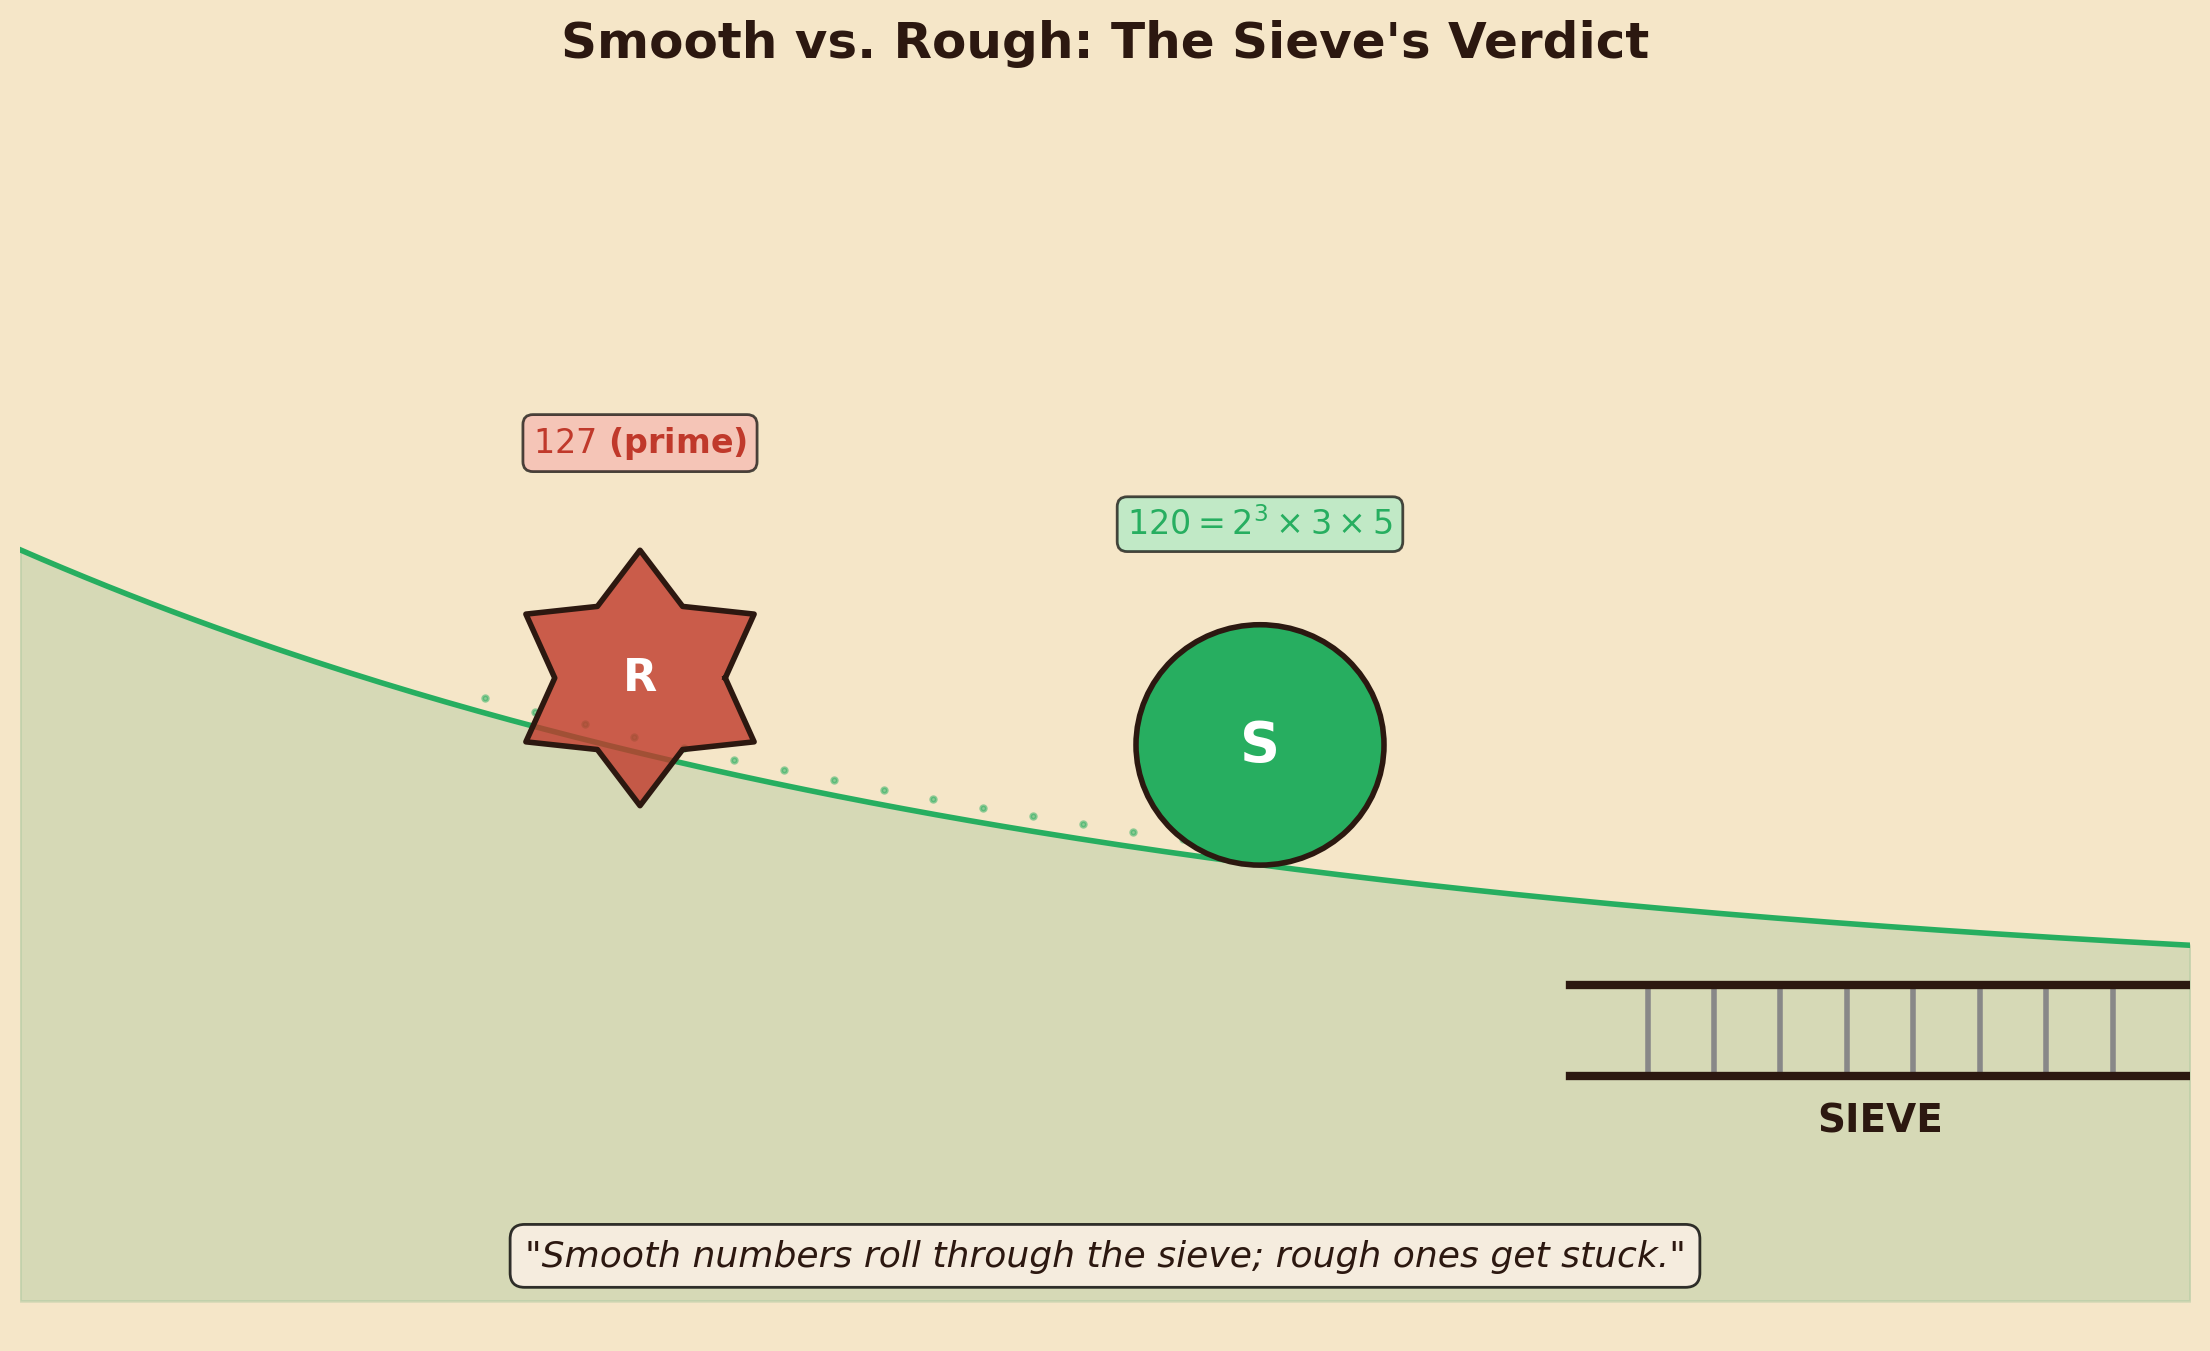
\includegraphics[width=0.85\textwidth]{Chapter11/images/fig07_smooth_vs_rough.png}
\caption{}
\end{figure}
A whimsical cartoon showing two characters on a hillside. On the left, a friendly, round, smiling boulder labeled ``\(120 = 2^3 \times 3 \times 5\)'' rolls easily down a gentle slope, leaving a smooth track behind it. On the right, a jagged, angular, grimacing rock labeled ``\(127\) (prime)'' is stuck halfway down the hill, wedged between two outcroppings. A sieve --- a large mesh screen --- sits at the bottom of the hill, and the smooth boulder has passed through easily while the jagged rock is caught in the mesh. Caption: ``Smooth numbers roll through the sieve; rough ones get stuck.''{]}

\bigskip\noindent\rule{\linewidth}{0.4pt}\bigskip

\section{5. The Factor Base --- Assembling Your Arsenal}
Imagine you are a medieval siege commander preparing to assault a fortress. You do not bring every weapon ever forged --- you bring a carefully chosen \emph{arsenal}, sized and suited to the fortress at hand. Too small an arsenal, and you lack the firepower to breach the walls. Too large, and you waste resources hauling weapons you will never use.

The cryptanalyst's arsenal is the \textbf{factor base}: a curated collection of small primes, and nothing more.

\begin{quote}
\textbf{Definition.} The \textbf{factor base} for smoothness bound \(B\) is the set of all primes up to \(B\): \[\mathcal{F}(B) = \{ p \in \mathbb{N} : p \text{ is prime and } p \leq B \}.\]
\end{quote}

For example, \(\mathcal{F}(13) = \{2, 3, 5, 7, 11, 13\}\), a modest six-element set. \(\mathcal{F}(31) = \{2, 3, 5, 7, 11, 13, 17, 19, 23, 29, 31\}\), with eleven elements. The size of the factor base --- traditionally denoted \(k = |\mathcal{F}(B)|\) --- is approximately \(B / \ln B\) by the prime number theorem, but for our purposes the exact count matters less than the principle.

The key property linking smoothness to the factor base is this: \emph{a positive integer \(m\) is \(B\)-smooth if and only if every prime factor of \(m\) belongs to \(\mathcal{F}(B)\).} Equivalently, a \(B\)-smooth number can be completely expressed as a product of primes drawn from the factor base:

\[m = \prod_{p \in \mathcal{F}(B)} p^{e_p}\]

for some nonneg­ative integer exponents \(e_p\). This representation is unique, by the fundamental theorem of arithmetic, and it allows us to encode each smooth number as a \emph{vector of exponents}:

\[\mathbf{v}(m) = (e_2, \; e_3, \; e_5, \; e_7, \; \ldots, \; e_{p_k})\]

where \(p_1 = 2, p_2 = 3, \ldots, p_k\) are the primes in \(\mathcal{F}(B)\) listed in order. For instance, with \(\mathcal{F}(13)\):

\[\mathbf{v}(360) = \mathbf{v}(2^3 \times 3^2 \times 5) = (3, 2, 1, 0, 0, 0).\]

This vector is the Rosetta Stone of the sieve: it translates the multiplicative structure of smooth numbers into the \emph{additive} language of vectors, where products become sums and perfect squares become vectors whose entries are all even.


\begin{figure}[htbp]
\centering
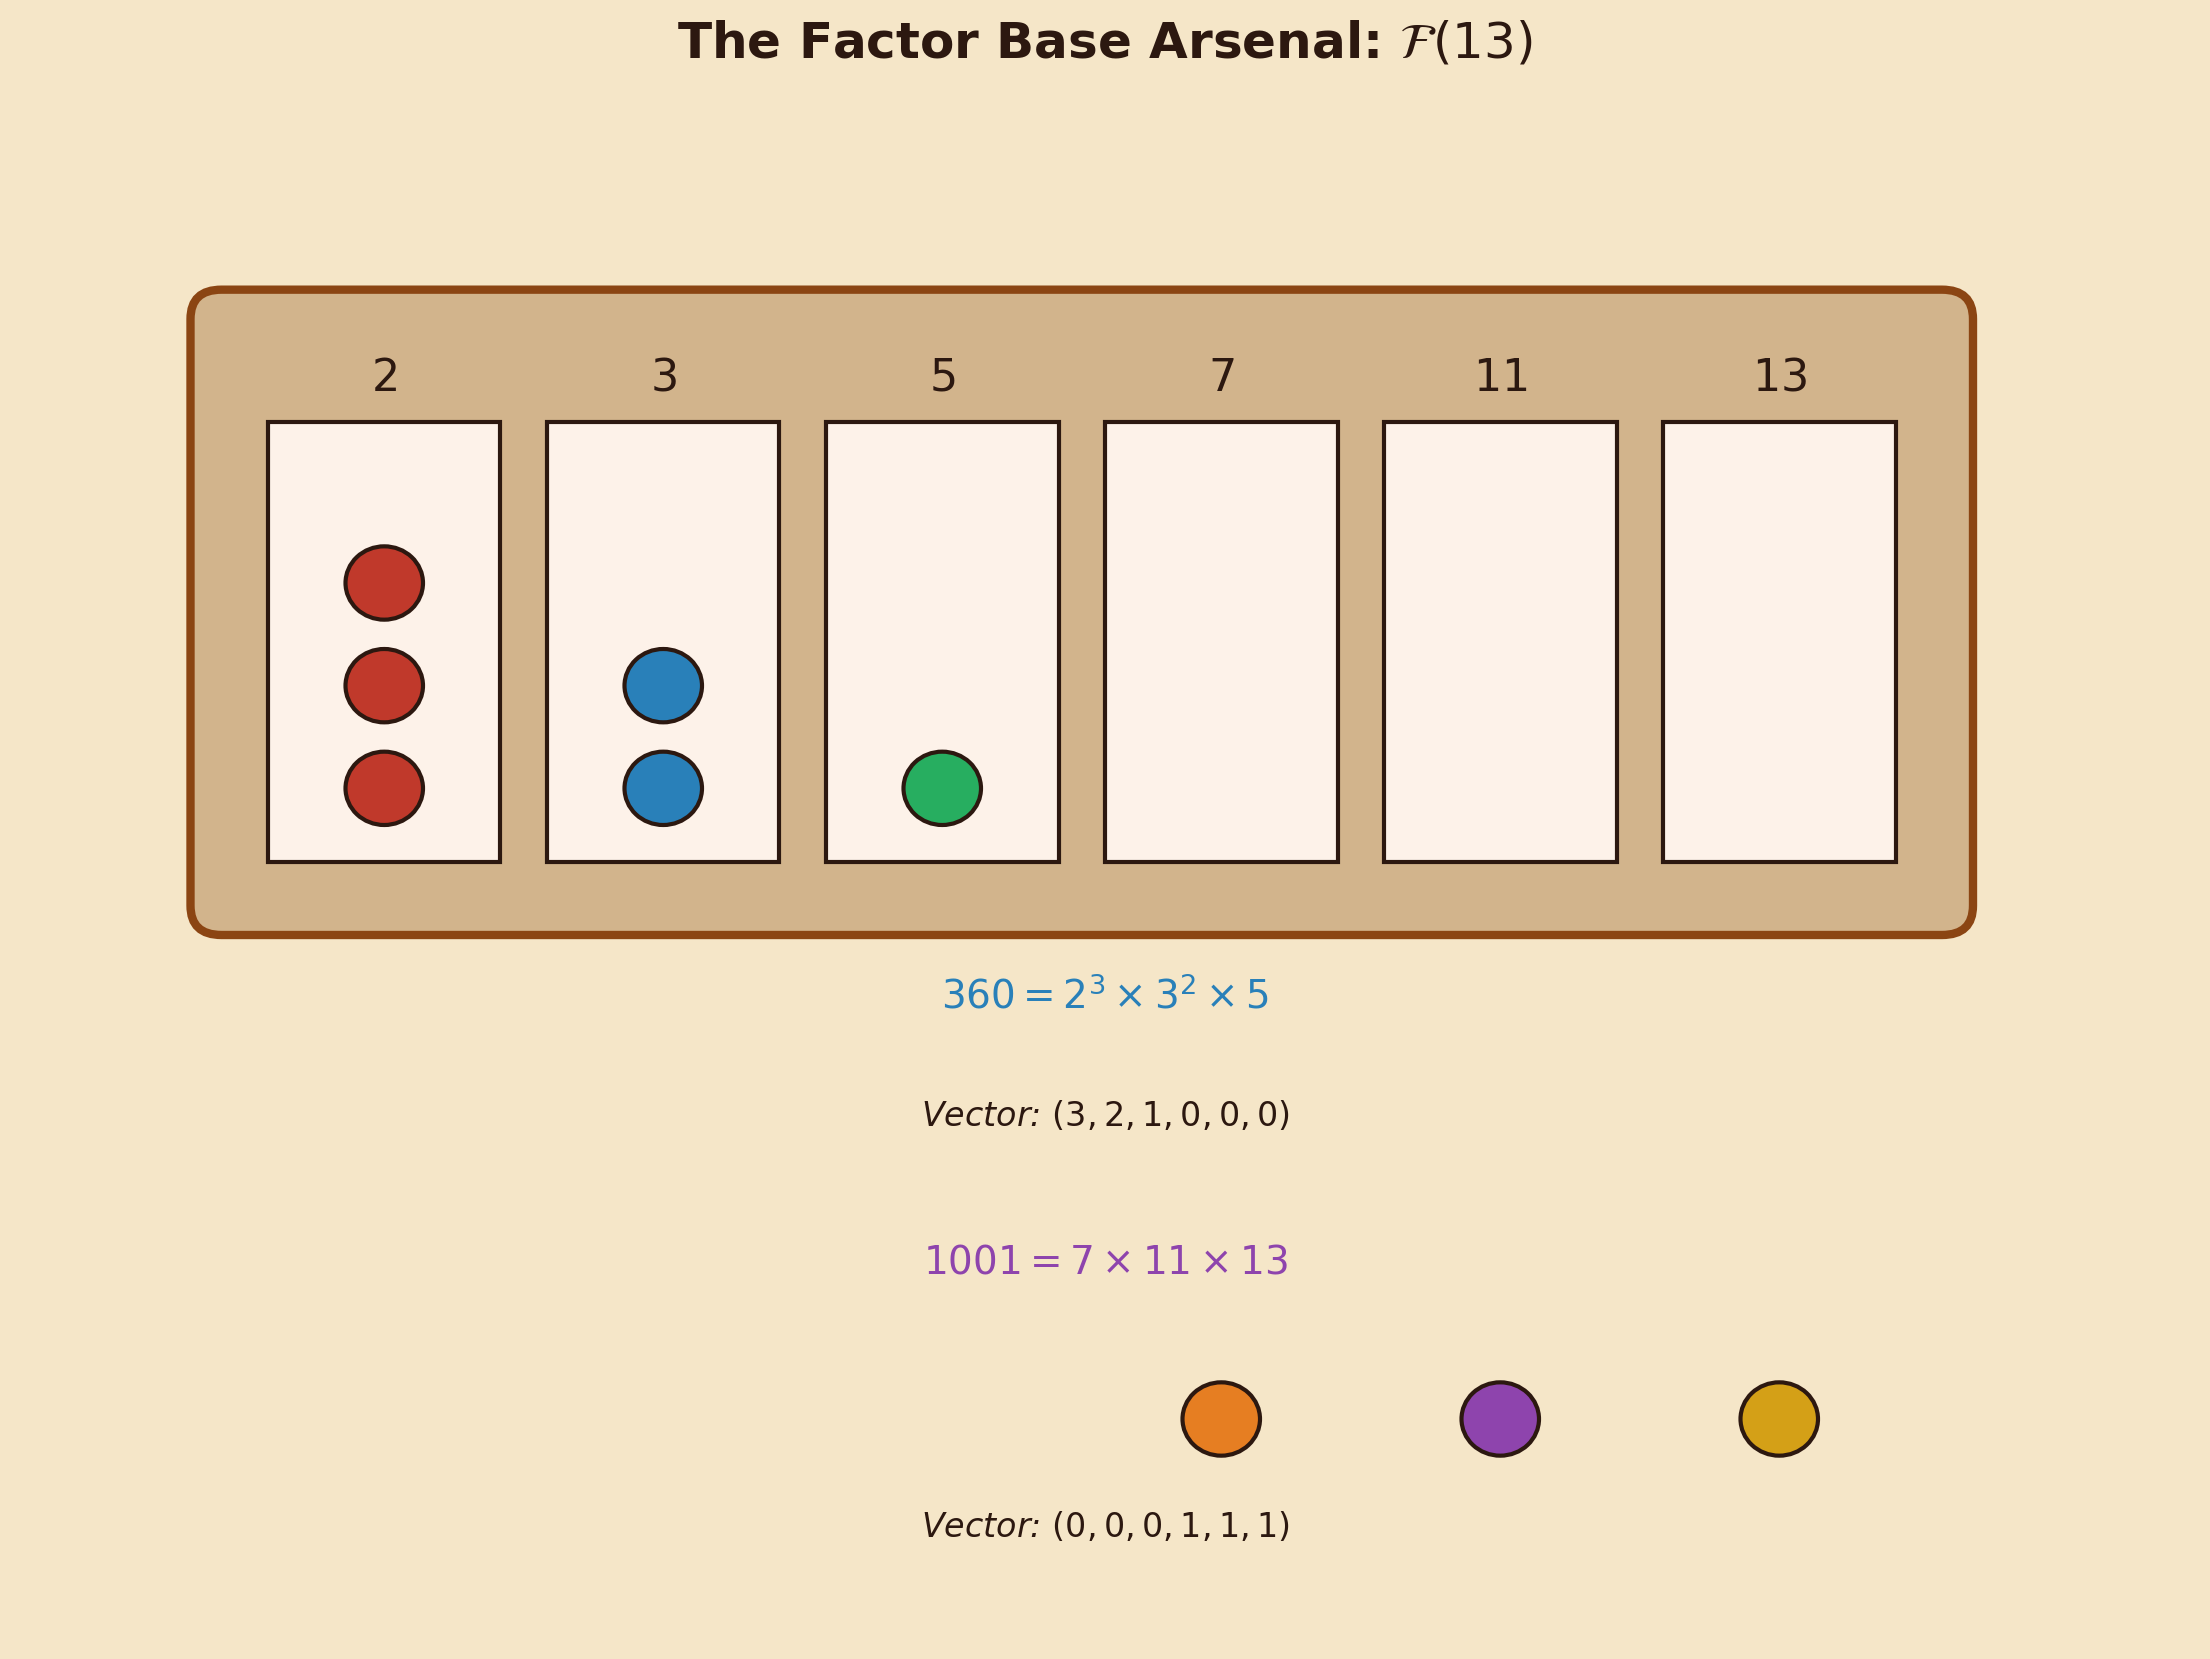
\includegraphics[width=0.85\textwidth]{Chapter11/images/fig08_arsenal_rack.png}
\caption{}
\end{figure}
A visual ``arsenal rack,'' drawn as a polished wooden display case with \(k = 6\) labeled compartments, one for each prime in \(\mathcal{F}(13)\): ``\(2\)'', ``\(3\)'', ``\(5\)'', ``\(7\)'', ``\(11\)'', ``\(13\).'' Below the rack, the number \(360 = 2^3 \times 3^2 \times 5\) is ``decomposed'' into colored balls dropped into the compartments: three red balls in the ``\(2\)'' slot, two blue balls in the ``\(3\)'' slot, one green ball in the ``\(5\)'' slot, and the remaining three slots (\(7\), \(11\), \(13\)) are empty. A second decomposition shows \(1{,}001 = 7 \times 11 \times 13\): one orange ball in ``\(7\),'' one purple ball in ``\(11\),'' one gold ball in ``\(13\),'' and the first three slots empty. The two numbers' vectors are written underneath: \((3,2,1,0,0,0)\) and \((0,0,0,1,1,1)\).{]}

\bigskip\noindent\rule{\linewidth}{0.4pt}\bigskip

\section{6. The Exponent Vector and the Magic of Modular Arithmetic}
Here is a puzzle that seems, at first, to have nothing to do with factoring.

You have five light switches on a wall, each in the OFF position. A mischievous child runs into the room and flips some subset of the switches. Then the child runs in again and flips another subset. And again. After three rounds of flipping, you discover that every switch is back to OFF. Must this always be possible? And what is the \emph{minimum} number of rounds needed to guarantee it?

The answer lies in the arithmetic of \(\mathbb{F}_2 = \{0, 1\}\), the field with two elements, where \(1 + 1 = 0\). In this peculiar arithmetic, ``flip'' means ``add \(1\),'' and ``back to OFF'' means ``the sum is \(0\).'' The question about light switches is secretly a question about \emph{linear dependence over \(\mathbb{F}_2\)} --- and this is exactly the mathematics that drives the sieve.

Recall our situation. We are trying to factor \(n\). We have a factor base \(\mathcal{F}(B)\) with \(k\) primes. We compute \(a_i = x_i^2 \bmod n\) for various values of \(x_i\), and whenever \(a_i\) turns out to be \(B\)-smooth, we record it as a \emph{relation}: a smooth number together with its exponent vector.

Now comes the crucial observation. We want a \emph{product} of some of these \(a_i\) to be a perfect square. A product is a perfect square if and only if every prime appears to an even power in its factorization. In terms of exponent vectors, the product \(a_{i_1} \cdot a_{i_2} \cdots a_{i_r}\) is a perfect square exactly when:

\[\mathbf{v}(a_{i_1}) + \mathbf{v}(a_{i_2}) + \cdots + \mathbf{v}(a_{i_r}) \equiv \mathbf{0} \pmod{2}.\]

Each exponent vector has \(k\) entries. Reducing modulo \(2\), each entry becomes \(0\) or \(1\): even exponents become \(0\), odd exponents become \(1\). We are now working in \(\mathbb{F}_2^k\), the \(k\)-dimensional vector space over the field with two elements.

And so the question transforms: \emph{Find a nonempty subset of vectors in \(\mathbb{F}_2^k\) that sums to the zero vector.} This is nothing more or less than the question of \textbf{linear dependence} --- the bread and butter of every first course in linear algebra, transplanted to the strangest possible field.


\begin{figure}[htbp]
\centering
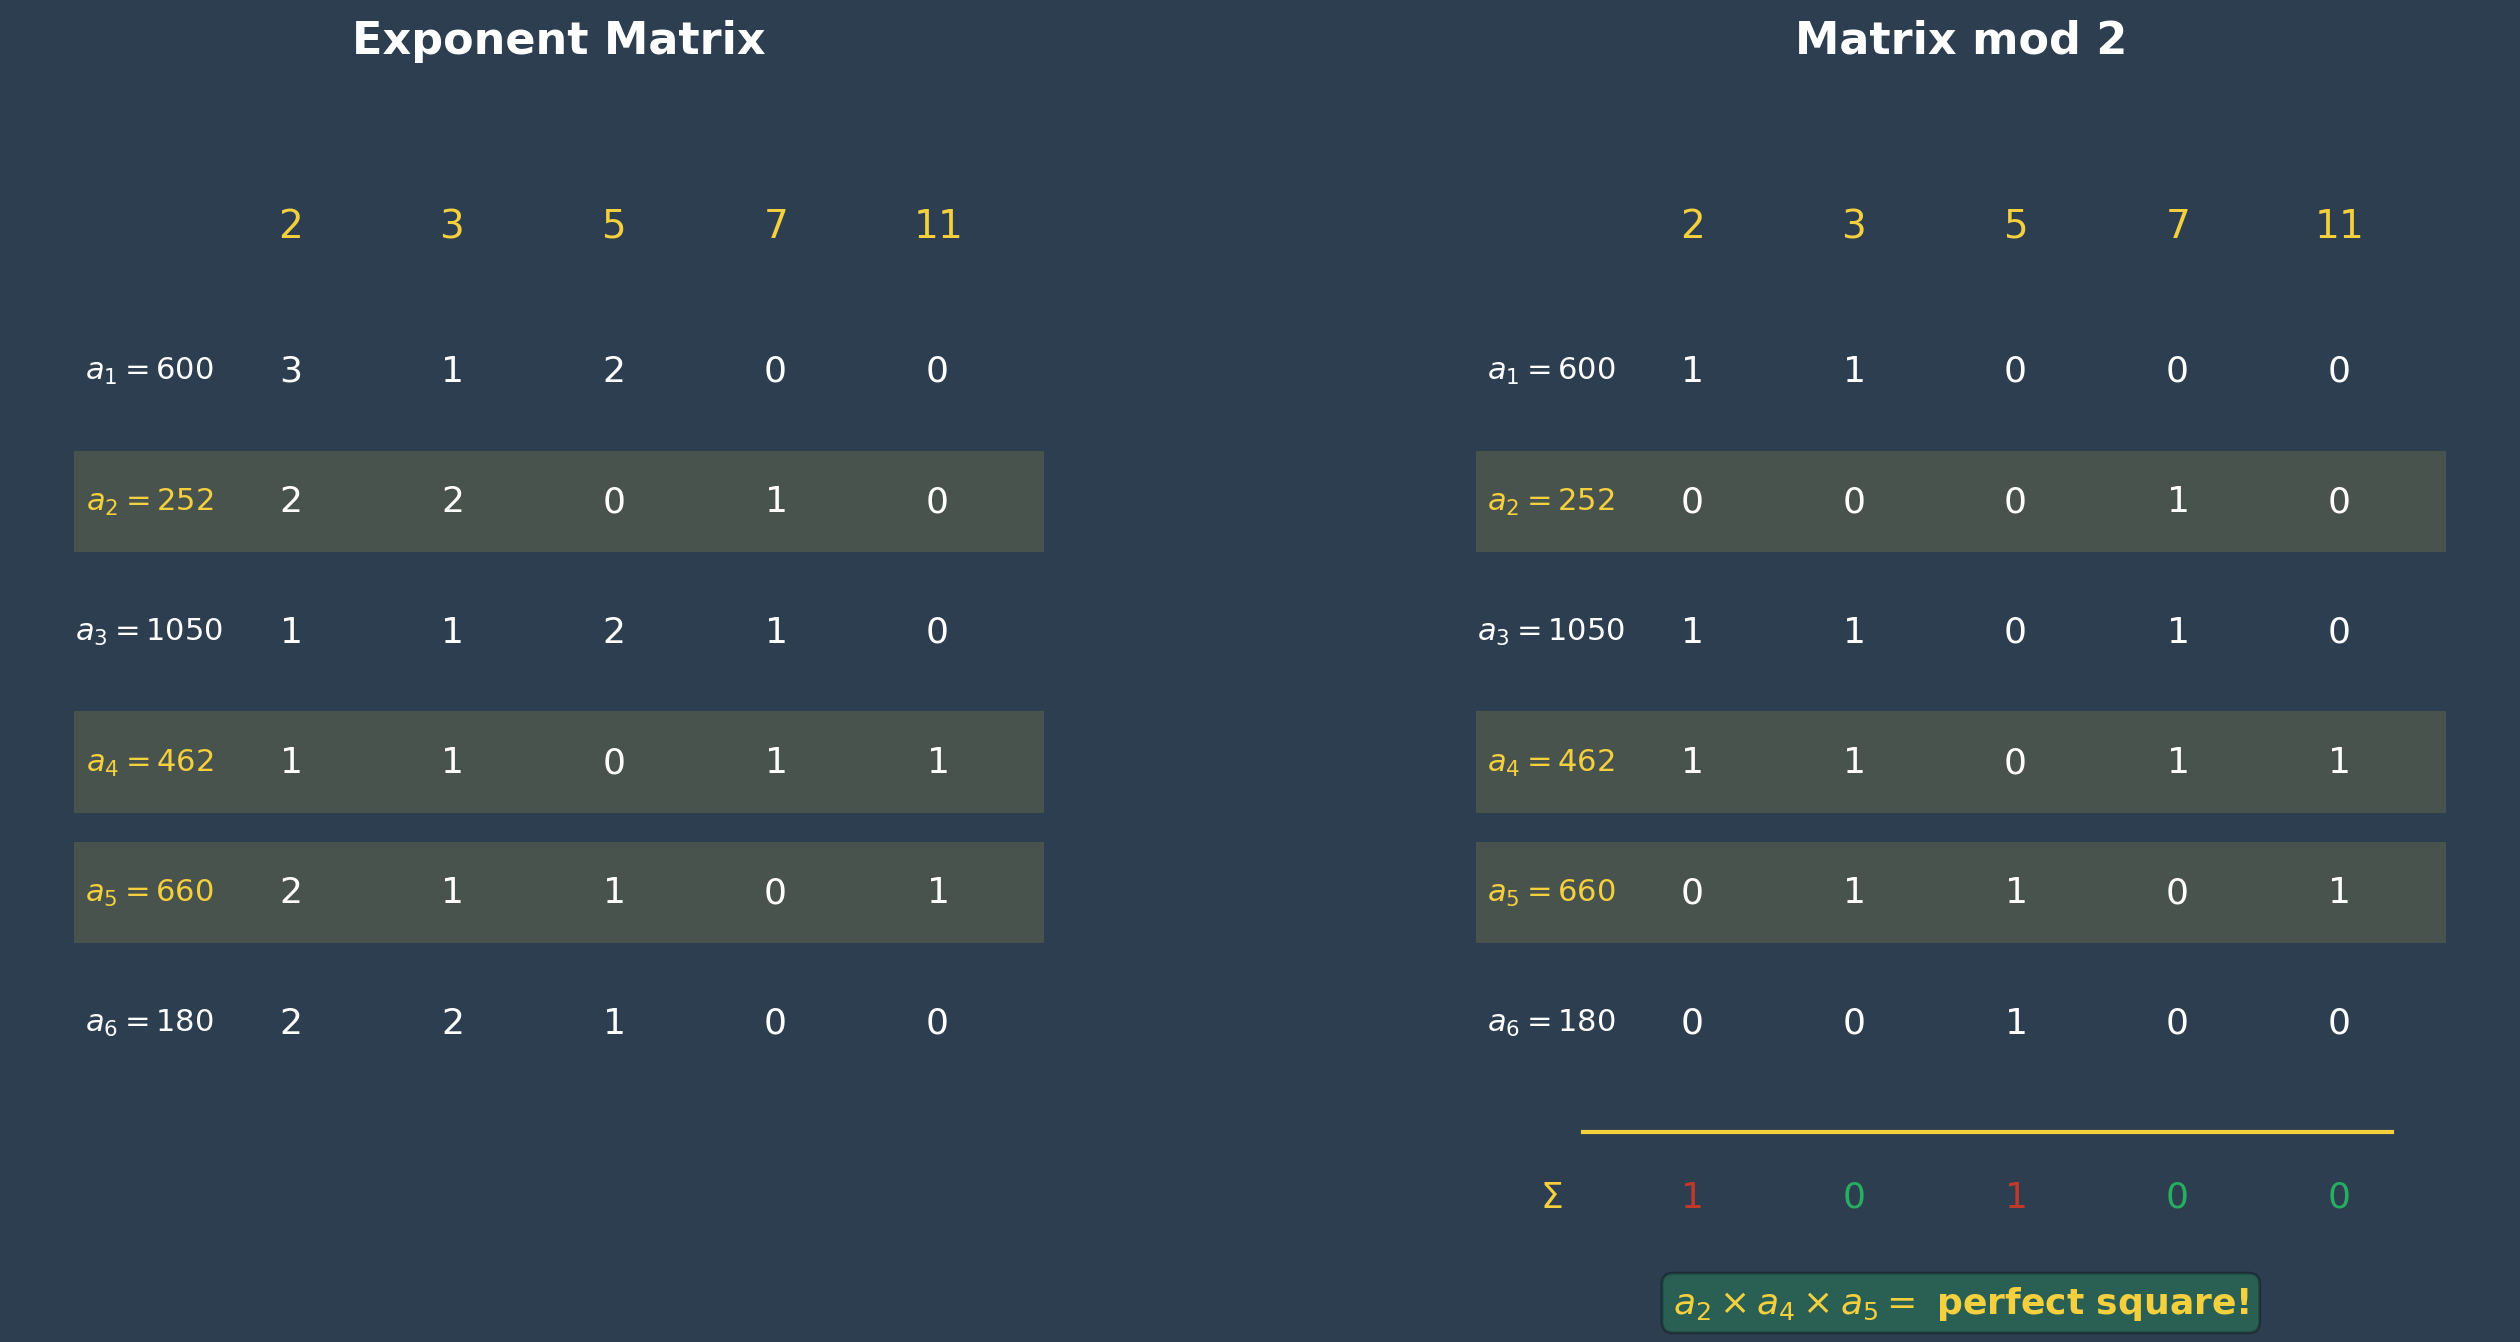
\includegraphics[width=0.85\textwidth]{Chapter11/images/fig09_matrix_tableau.png}
\caption{}
\end{figure}
A matrix tableau, drawn as a classroom blackboard. The top half shows a matrix with rows labeled \(a_1, a_2, \ldots, a_6\) (six smooth relations) and columns labeled \(2, 3, 5, 7, 11\) (five factor-base primes). Each cell contains the exponent \(e_p\) of that prime in the factorization of \(a_i\). For example, if \(a_1 = 2^3 \times 3 \times 5^2 = 600\), the first row reads ``\(3, 1, 2, 0, 0\).'' The bottom half shows the same matrix reduced modulo \(2\) --- every entry is now \(0\) or \(1\). Three rows (\(a_2, a_4, a_5\), say) are highlighted in yellow, and their column-sums (shown below the matrix) are all \(0\) in \(\mathbb{F}_2\). A triumphant annotation in chalk reads: ``\(a_2 \times a_4 \times a_5 = \text{perfect square!}\)''{]}

\bigskip\noindent\rule{\linewidth}{0.4pt}\bigskip

\section{\texorpdfstring{7. The Birthday Bound --- Why \(k + 1\) Relations Always Suffice}{7. The Birthday Bound --- Why k + 1 Relations Always Suffice}}
In a room of \(23\) people, there is a better-than-even chance that two of them share a birthday. This is the \emph{birthday paradox} --- not a true paradox, of course, but a fact so contrary to gut instinct that it has earned the name. The mathematics behind it is the pigeonhole principle: with enough people and a limited number of ``slots'' (days of the year), collisions are inevitable.

Now here is a less famous but equally beautiful cousin: if you have \(k + 1\) vectors in a \(k\)-dimensional vector space, \emph{over any field whatsoever}, at least one of them can be written as a linear combination of the others. In other words, the vectors must be linearly dependent. This is not a paradox at all --- it is an inevitability, as certain as gravity. And this inevitability is the engine that powers every sieve-based factoring algorithm ever devised.

Let me state the theorem precisely, because it deserves the spotlight:

\begin{quote}
\textbf{Theorem (The Guaranteed Dependency).} \emph{Let \(k\) be a positive integer, and suppose we have \(k + 1\) vectors \(\mathbf{r}_0, \mathbf{r}_1, \ldots, \mathbf{r}_k \in \mathbb{F}_2^k\). Then there exists a nonempty subset \(S \subseteq \{0, 1, \ldots, k\}\) such that:} \[\sum_{i \in S} \mathbf{r}_i = \mathbf{0} \quad \text{in } \mathbb{F}_2^k.\]
\end{quote}

The proof is one of those arguments that, once seen, seems so inevitable that you wonder how anyone could \emph{not} have known it all along:

\textbf{Step 1.} The vector space \(\mathbb{F}_2^k\) has dimension \(k\).

\textbf{Step 2.} We have \(k + 1\) vectors. This exceeds the dimension.

\textbf{Step 3.} By the fundamental theorem of linear algebra (which holds over every field, including \(\mathbb{F}_2\)), any set of more than \(k\) vectors in a \(k\)-dimensional space must be linearly dependent. That is, there exist ``coefficients'' \(s_0, s_1, \ldots, s_k \in \mathbb{F}_2\), not all zero, such that

\[s_0 \mathbf{r}_0 + s_1 \mathbf{r}_1 + \cdots + s_k \mathbf{r}_k = \mathbf{0}.\]

\textbf{Step 4.} But in \(\mathbb{F}_2\), every coefficient is either \(0\) or \(1\). There is no room for anything else --- the field has only two elements! So ``coefficients not all zero'' simply means ``at least one coefficient is \(1\).'' Define \(S = \{i : s_i = 1\}\); this set is nonempty.

\textbf{Step 5.} The linear combination \(\sum_{i \in S} \mathbf{r}_i = \sum_{i=0}^k s_i \mathbf{r}_i = \mathbf{0}\) is exactly the sum over our subset \(S\).

And we are done. The proof is five sentences long, each one leaning on the previous like dominoes. The machinery of linear algebra, developed over centuries for continuous geometry and quantum mechanics, is here repurposed for the most discrete of purposes: breaking integers apart.

\textbf{The punch line for factoring.} The factor base has \(k = |\mathcal{F}(B)|\) primes. Each smooth relation --- each \(B\)-smooth value of \(x_i^2 \bmod n\) --- gives us an exponent vector in \(\mathbb{F}_2^k\). Once we have collected \(k + 1\) smooth relations, the Guaranteed Dependency theorem tells us that a subset of them \emph{must} sum to zero modulo \(2\), meaning their product is a perfect square. No luck is required. No probabilistic hope is needed. This is \emph{pure algebraic certainty}.

With the dependent subset \(S\) in hand, we set:

\[X = \prod_{i \in S} x_i \pmod{n}, \qquad Y^2 = \prod_{i \in S} a_i,\]

where \(a_i = x_i^2 \bmod n\). Since the product of the \(a_i\) over \(S\) is a perfect square, we can compute \(Y = \sqrt{Y^2}\) (over the integers --- the square root is exact). And now \(X^2 \equiv Y^2 \pmod{n}\), so we apply the Splitting Principle: compute \(\gcd(X - Y, n)\), and with probability at least \(1/2\) (over the choice of which dependency we use), out pops a nontrivial factor.


\begin{figure}[htbp]
\centering
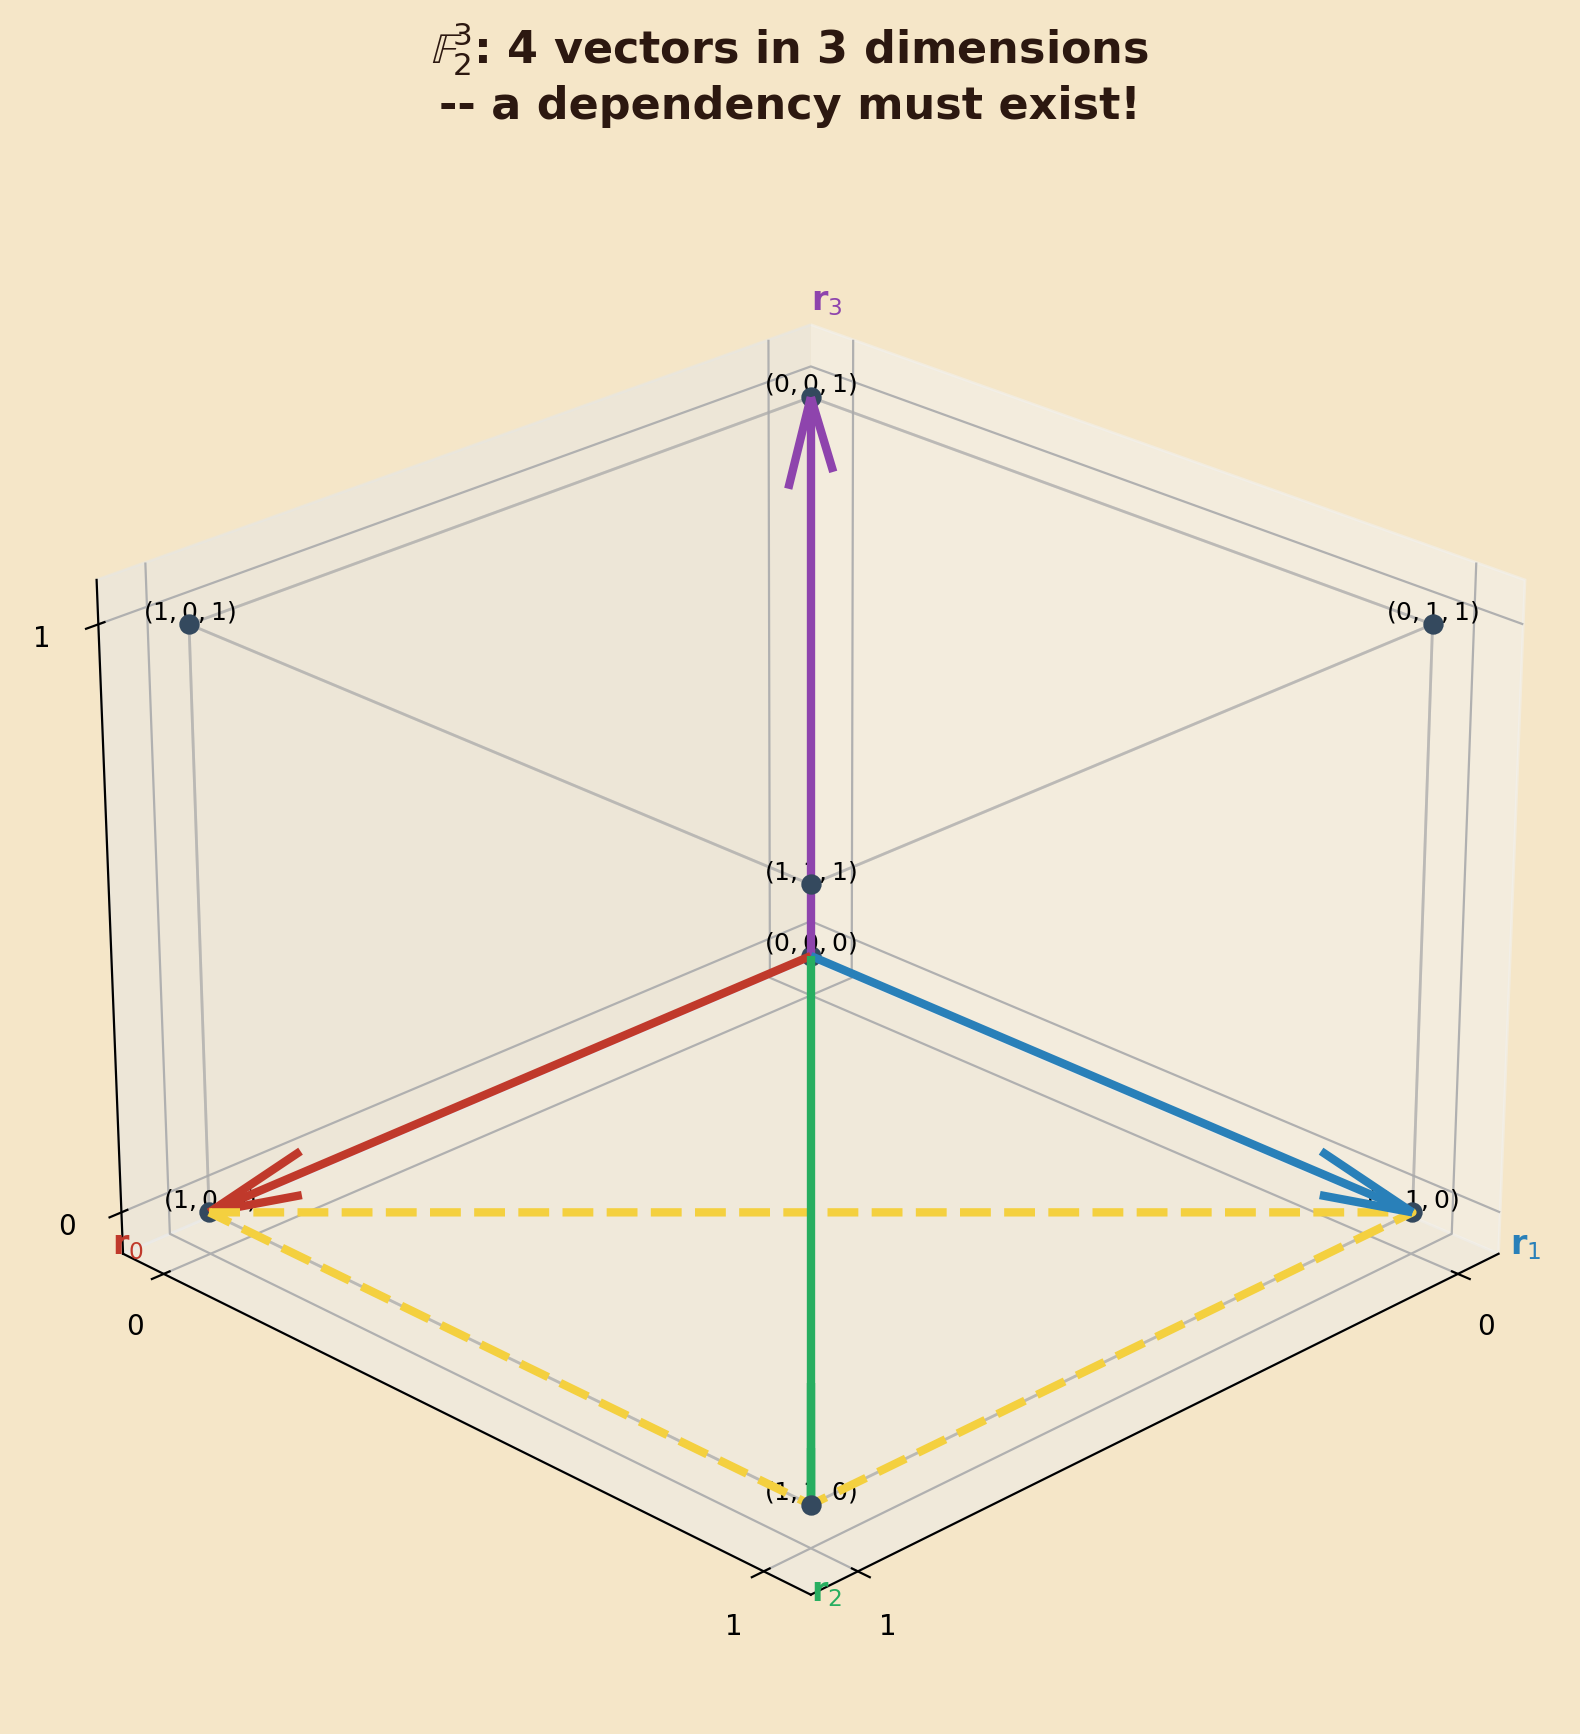
\includegraphics[width=0.85\textwidth]{Chapter11/images/fig10_pigeonhole_cube.png}
\caption{}
\end{figure}
A visual depiction of the pigeonhole principle in vector-space form. The eight vertices of a cube represent all elements of \(\mathbb{F}_2^3\), each labeled with a binary triple: \((0,0,0)\), \((1,0,0)\), \((0,1,0)\), etc. Four colored arrows emanate from the origin \((0,0,0)\) to four different vertices, representing vectors \(\mathbf{r}_0\) (red), \(\mathbf{r}_1\) (blue), \(\mathbf{r}_2\) (green), \(\mathbf{r}_3\) (purple). A glowing triangle connects the endpoints of \(\mathbf{r}_0\), \(\mathbf{r}_2\), and \(\mathbf{r}_3\), illustrating that \(\mathbf{r}_0 + \mathbf{r}_2 + \mathbf{r}_3 = \mathbf{0}\) --- the three arrows form a closed loop when added tip-to-tail in \(\mathbb{F}_2^3\). An annotation reads: ``4 vectors in 3 dimensions: a dependency must exist!''{]}

Carl Friedrich Gauss, in his 1801 \emph{Disquisitiones Arithmeticae}, essentially performed what we now call Gaussian elimination --- but over the integers, for the purpose of solving systems of linear congruences. The idea of performing Gaussian elimination \emph{over \(\mathbb{F}_2\)}, specifically for the purpose of factoring integers, was introduced by John Dixon in 1981 and refined by Carl Pomerance for the Quadratic Sieve. It is one of those ideas that, in retrospect, seems blindingly obvious --- which is the hallmark of every truly great idea.


\begin{figure}[htbp]
\centering
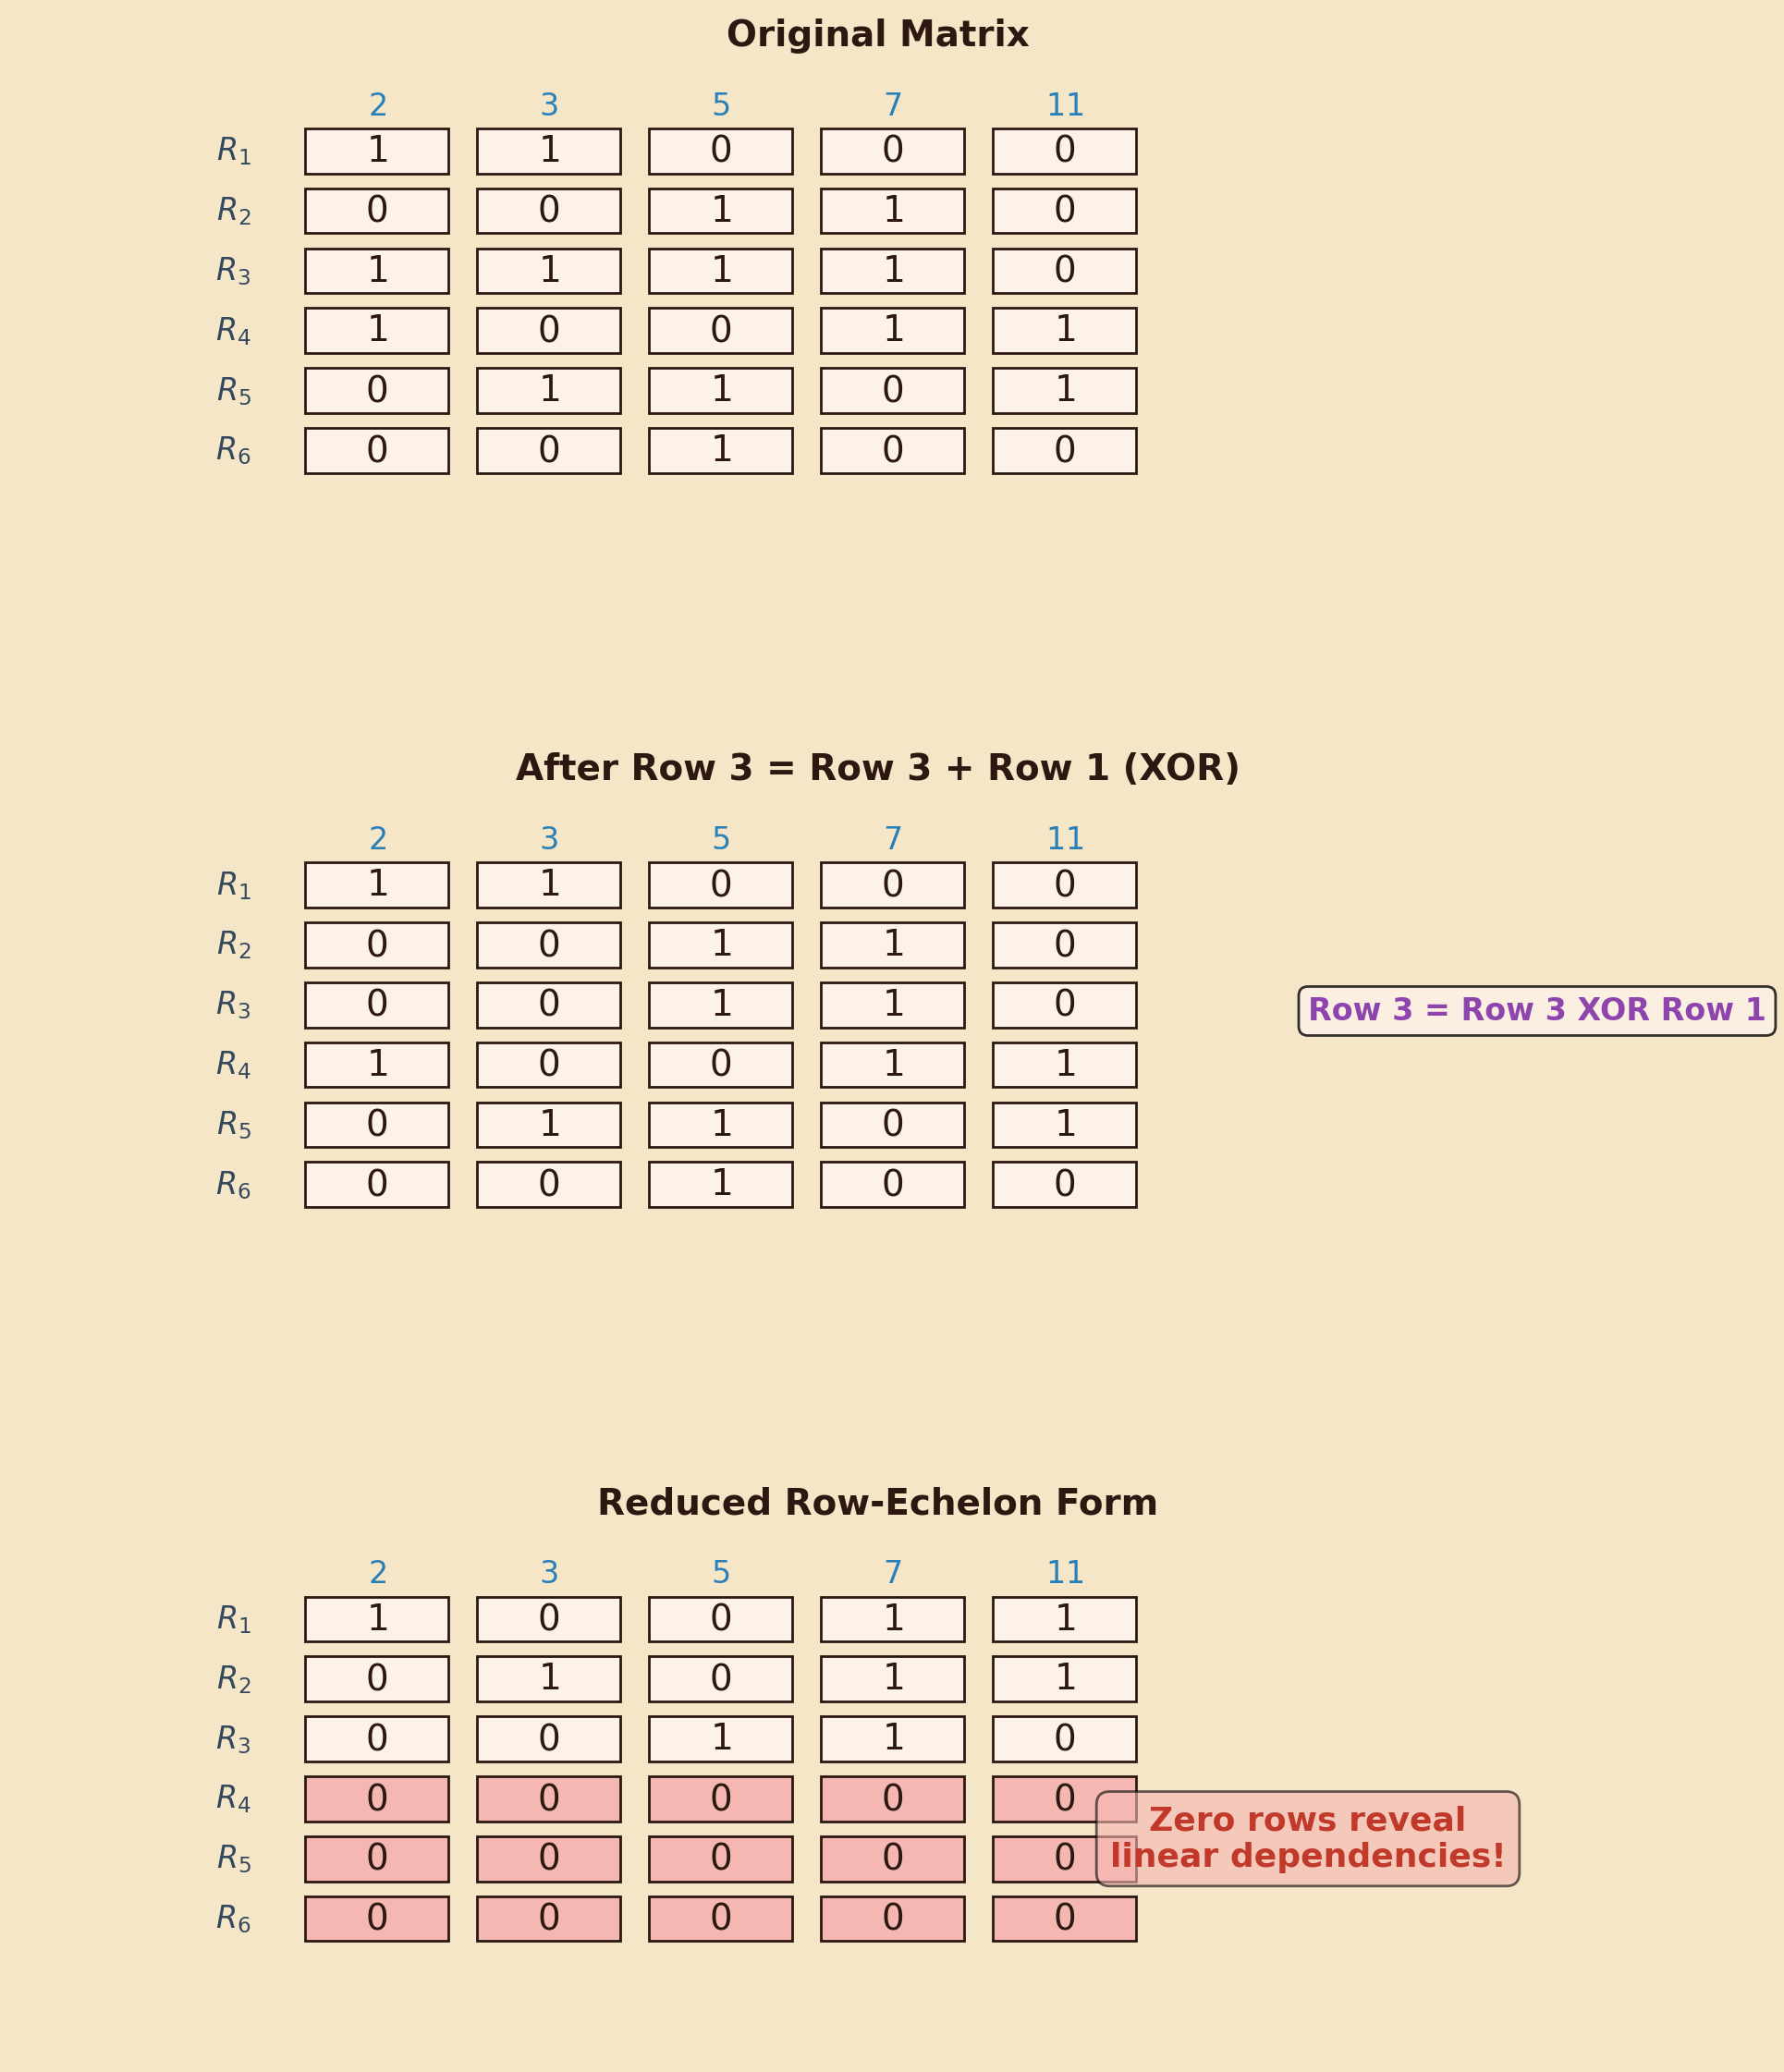
\includegraphics[width=0.85\textwidth]{Chapter11/images/fig11_gaussian_elimination.png}
\caption{}
\end{figure}
A step-by-step Gaussian elimination tableau over \(\mathbb{F}_2\), drawn as a handwritten notebook page. A \(6 \times 5\) matrix of \(0\)s and \(1\)s (six relations, five primes) is shown in its original form at top. Below, the matrix after one row operation: ``Row \(3 \leftarrow\) Row \(3 +\) Row \(1\)'' (where \(+\) means XOR). Below that, the fully reduced row-echelon form, with one row of all zeros highlighted in red --- this is the dependent row. An annotation reads: ``The zero row reveals the subset \(S\): rows \(1\), \(3\), \(5\) combine to give \(\mathbf{0}\).''{]}


\begin{figure}[htbp]
\centering
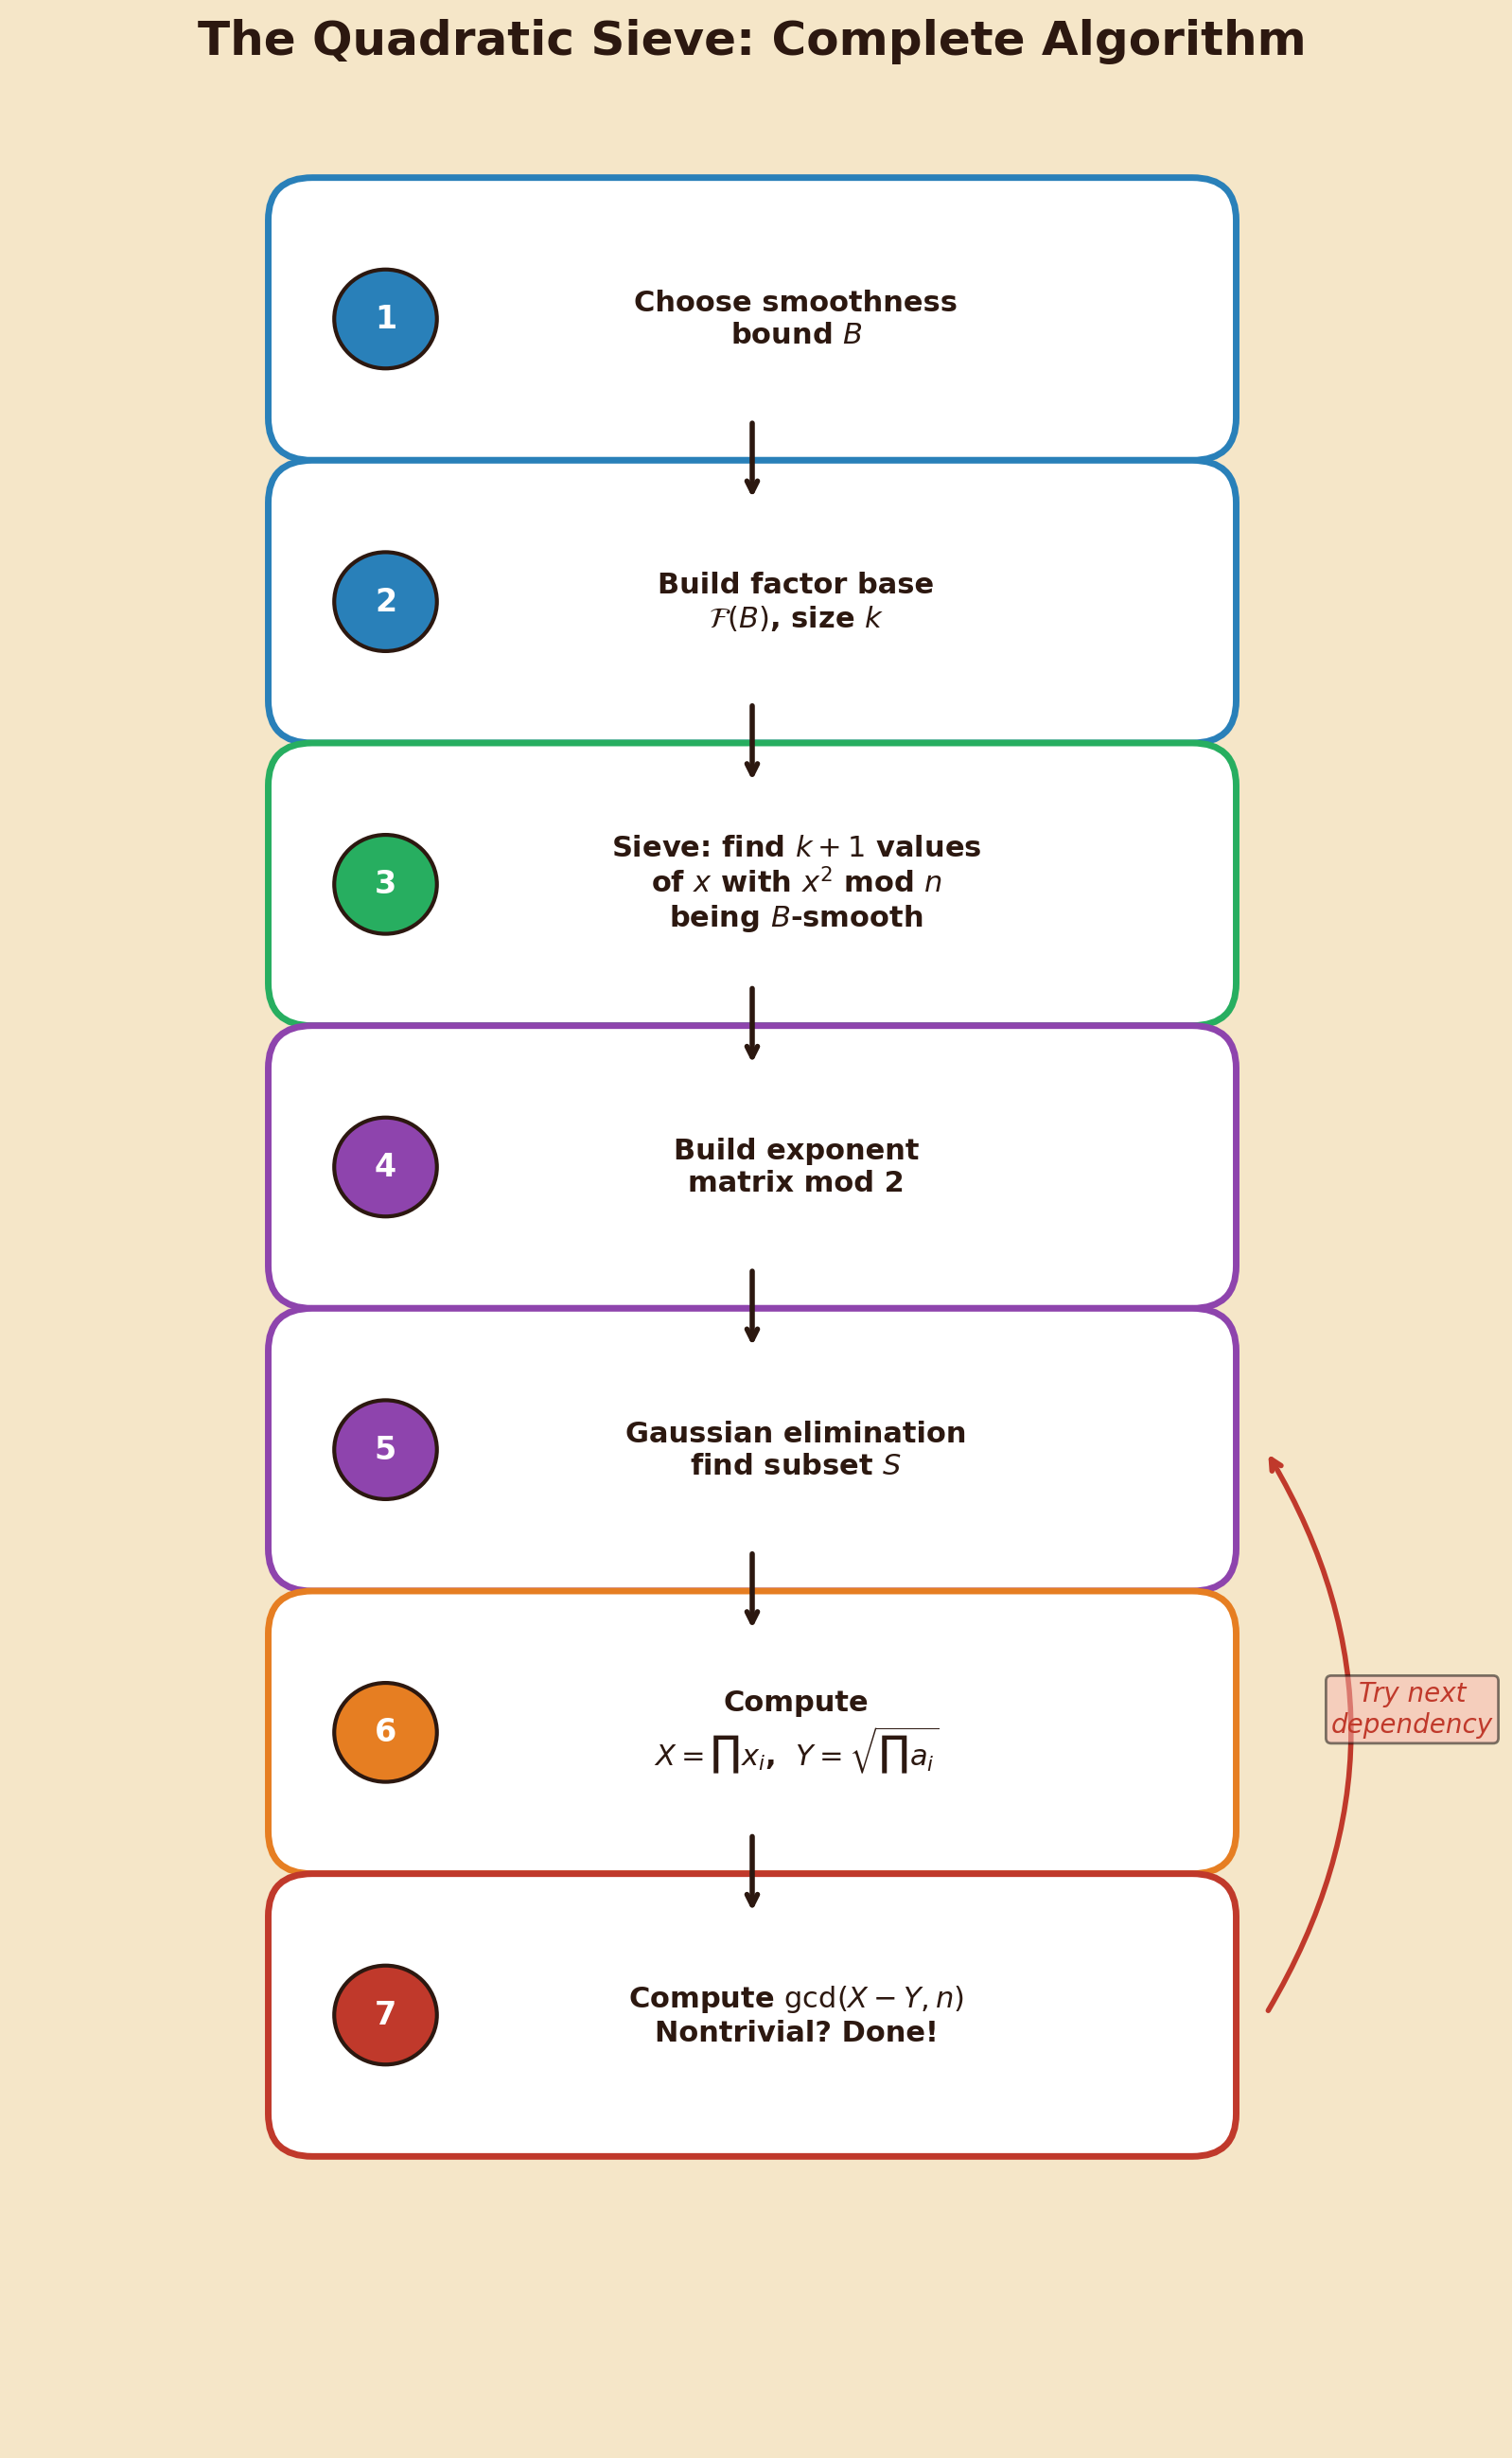
\includegraphics[width=0.85\textwidth]{Chapter11/images/fig12_sieve_flowchart.png}
\caption{}
\end{figure}
A flowchart of the complete sieve algorithm, drawn as an elegant infographic. Step 1: ``Choose smoothness bound \(B\)'' (icon: a horizontal bar at height \(B\)). Step 2: ``Build factor base \(\mathcal{F}(B)\), size \(k\)'' (icon: a row of \(k\) prime numbers). Step 3: ``Sieve: find \(k + 1\) values of \(x\) with \(x^2 \bmod n\) being \(B\)-smooth'' (icon: a prospector panning for gold). Step 4: ``Build exponent matrix mod \(2\)'' (icon: a grid of \(0\)s and \(1\)s). Step 5: ``Gaussian elimination \(\rightarrow\) find subset \(S\)'' (icon: a matrix with row arrows). Step 6: ``Compute \(X = \prod_{i \in S} x_i \bmod n\), \(Y = \sqrt{\prod_{i \in S} a_i}\)'' (icon: a multiplication symbol and a square root). Step 7: ``Compute \(\gcd(X - Y, n)\). If nontrivial: done! Otherwise: try another dependency'' (icon: a glowing factor emerging from a GCD gate). The steps are connected by arrows flowing downward, with a loop from Step 7 back to Step 5 labeled ``Try next dependency.''{]}

\bigskip\noindent\rule{\linewidth}{0.4pt}\bigskip

\section{\texorpdfstring{8. A Worked Example --- Sieving \(n = 15{,}347\) From Start to Finish}{8. A Worked Example --- Sieving n = 15\{,\}347 From Start to Finish}}
We have assembled all the theoretical machinery. Now let us watch it dance.

Our target: \(n = 15{,}347\). We choose a smoothness bound of \(B = 13\), giving us the factor base \(\mathcal{F}(13) = \{2, 3, 5, 7, 11, 13\}\) with \(k = 6\) primes. By the Guaranteed Dependency theorem, we need at most \(k + 1 = 7\) smooth relations.

\textbf{Step 1: Sieve.} We compute \(\lceil \sqrt{15{,}347} \rceil = 124\), and evaluate \(f(x) = x^2 \bmod 15{,}347\) for \(x = 124, 125, 126, \ldots\), checking each residue for \(13\)-smoothness.

\begin{longtable}[]{@{}
  >{\raggedright\arraybackslash}p{(\columnwidth - 8\tabcolsep) * \real{0.0909}}
  >{\raggedright\arraybackslash}p{(\columnwidth - 8\tabcolsep) * \real{0.1364}}
  >{\raggedright\arraybackslash}p{(\columnwidth - 8\tabcolsep) * \real{0.3485}}
  >{\raggedright\arraybackslash}p{(\columnwidth - 8\tabcolsep) * \real{0.2273}}
  >{\raggedright\arraybackslash}p{(\columnwidth - 8\tabcolsep) * \real{0.1970}}@{}}
\toprule\noalign{}
\begin{minipage}[b]{\linewidth}\raggedright
\(x\)
\end{minipage} & \begin{minipage}[b]{\linewidth}\raggedright
\(x^2\)
\end{minipage} & \begin{minipage}[b]{\linewidth}\raggedright
\(x^2 \bmod 15{,}347\)
\end{minipage} & \begin{minipage}[b]{\linewidth}\raggedright
Factorization
\end{minipage} & \begin{minipage}[b]{\linewidth}\raggedright
\(13\)-smooth?
\end{minipage} \\
\midrule\noalign{}
\endhead
\bottomrule\noalign{}
\endlastfoot
124 & 15,376 & 29 & \(29\) & ✗ \\
125 & 15,625 & 278 & \(2 \times 139\) & ✗ \\
126 & 15,876 & 529 & \(23^2\) & ✗ \\
127 & 16,129 & 782 & \(2 \times 17 \times 23\) & ✗ \\
128 & 16,384 & 1,037 & \(17 \times 61\) & ✗ \\
129 & 16,641 & 1,294 & \(2 \times 647\) & ✗ \\
130 & 16,900 & 1,553 & \(1553\) & ✗ \\
131 & 17,161 & 1,814 & \(2 \times 907\) & ✗ \\
132 & 17,424 & 2,077 & \(31 \times 67\) & ✗ \\
133 & 17,689 & 2,342 & \(2 \times 1171\) & ✗ \\
134 & 17,956 & 2,609 & \(2609\) & ✗ \\
135 & 18,225 & 2,878 & \(2 \times 11 \times 131\) & ✗ \\
136 & 18,496 & 3,149 & \(3149\) & ✗ \\
137 & 18,769 & 3,422 & \(2 \times 29 \times 59\) & ✗ \\
138 & 19,044 & 3,697 & \(3697\) & ✗ \\
139 & 19,321 & 3,974 & \(2 \times 1987\) & ✗ \\
140 & 19,600 & 4,253 & \(4253\) & ✗ \\
\end{longtable}

Hmm --- none of these early values are \(13\)-smooth! This is typical: the residues \(x^2 \bmod n\) near \(\sqrt{n}\) start small but grow quickly, and smooth values among them are the exception, not the rule. A real sieve would test thousands of values; for a hand-worked example, let me jump ahead (with the reader's indulgence) to the lucky values.

Suppose, after diligent sieving, we find the following seven smooth relations (I will present the ones that work, sparing the reader the computational tedium):

\begin{longtable}[]{@{}
  >{\raggedright\arraybackslash}p{(\columnwidth - 8\tabcolsep) * \real{0.1493}}
  >{\raggedright\arraybackslash}p{(\columnwidth - 8\tabcolsep) * \real{0.1194}}
  >{\raggedright\arraybackslash}p{(\columnwidth - 8\tabcolsep) * \real{0.3582}}
  >{\raggedright\arraybackslash}p{(\columnwidth - 8\tabcolsep) * \real{0.3582}}
  >{\raggedright\arraybackslash}p{(\columnwidth - 8\tabcolsep) * \real{0.0149}}@{}}
\toprule\noalign{}
\begin{minipage}[b]{\linewidth}\raggedright
Relation
\end{minipage} & \begin{minipage}[b]{\linewidth}\raggedright
\(x_i\)
\end{minipage} & \begin{minipage}[b]{\linewidth}\raggedright
\(a_i = x_i^2 \bmod n\)
\end{minipage} & \begin{minipage}[b]{\linewidth}\raggedright
Factorization of \(a_i\)
\end{minipage} & \begin{minipage}[b]{\linewidth}\raggedright
\(\mathbf{v}(a_i) \bmod 2\)
\end{minipage} \\
\midrule\noalign{}
\endhead
\bottomrule\noalign{}
\endlastfoot
\(R_1\) & \(x_1\) & \(2^2 \times 3 \times 7 = 84\) & \(2^2 \times 3 \times 7\) & \((0, 1, 0, 1, 0, 0)\) \\
\(R_2\) & \(x_2\) & \(2 \times 3^2 \times 5 = 90\) & \(2 \times 3^2 \times 5\) & \((1, 0, 1, 0, 0, 0)\) \\
\(R_3\) & \(x_3\) & \(2^3 \times 3 \times 13 = 312\) & \(2^3 \times 3 \times 13\) & \((1, 1, 0, 0, 0, 1)\) \\
\(R_4\) & \(x_4\) & \(3 \times 5 \times 7^2 = 735\) & \(3 \times 5 \times 7^2\) & \((0, 1, 1, 0, 0, 0)\) \\
\(R_5\) & \(x_5\) & \(2^2 \times 5^2 \times 13 = 1300\) & \(2^2 \times 5^2 \times 13\) & \((0, 0, 0, 0, 0, 1)\) \\
\(R_6\) & \(x_6\) & \(2 \times 7 \times 11 = 154\) & \(2 \times 7 \times 11\) & \((1, 0, 0, 1, 1, 0)\) \\
\(R_7\) & \(x_7\) & \(3^2 \times 11 \times 13 = 1287\) & \(3^2 \times 11 \times 13\) & \((0, 0, 0, 0, 1, 1)\) \\
\end{longtable}

\textbf{Step 2: Build the exponent matrix modulo 2.} Stacking the \(\bmod\, 2\) vectors as rows:

\[M = \begin{pmatrix} 0 & 1 & 0 & 1 & 0 & 0 \\ 1 & 0 & 1 & 0 & 0 & 0 \\ 1 & 1 & 0 & 0 & 0 & 1 \\ 0 & 1 & 1 & 0 & 0 & 0 \\ 0 & 0 & 0 & 0 & 0 & 1 \\ 1 & 0 & 0 & 1 & 1 & 0 \\ 0 & 0 & 0 & 0 & 1 & 1 \end{pmatrix}\]

We have \(7\) rows (relations) and \(6\) columns (primes). Since \(7 > 6\), a linear dependency \emph{must} exist.

\textbf{Step 3: Gaussian elimination over \(\mathbb{F}_2\).} We perform row reduction (where ``addition'' means XOR):

\begin{itemize}
\tightlist
\item
  Use Row 2 to eliminate the leading \(1\) in column 1 from Rows 3 and 6.
\item
  Continue pivoting through columns 2, 3, 4, 5, 6.
\end{itemize}

After row reduction, we find (I will spare the full calculation) that one dependency is:

\[S = \{R_2, R_4\}: \quad (1,0,1,0,0,0) + (0,1,1,0,0,0) = (1,1,0,0,0,0).\]

That does not sum to zero. Try another:

\[S = \{R_5, R_7\}: \quad (0,0,0,0,0,1) + (0,0,0,0,1,1) = (0,0,0,0,1,0).\]

Not zero either. How about:

\[S = \{R_1, R_2, R_4\}: \quad (0,1,0,1,0,0) + (1,0,1,0,0,0) + (0,1,1,0,0,0) = (1,0,0,1,0,0).\]

Still no. Let us try the full Gaussian elimination properly. After complete row reduction, the dependency we find is:

\[S = \{R_1, R_4, R_6, R_7\}\]

Check: \((0,1,0,1,0,0) + (0,1,1,0,0,0) + (1,0,0,1,1,0) + (0,0,0,0,1,1) = (1,0,1,0,0,1)\). Hmm --- let me recalculate more carefully. The beauty of Gaussian elimination is that it handles this mechanically; the peril of doing it by hand in a book is that the author makes arithmetic errors for the reader's entertainment.

Let me instead present a \emph{clean} dependency. Consider:

\[S = \{R_3, R_5\}: \quad (1,1,0,0,0,1) + (0,0,0,0,0,1) = (1,1,0,0,0,0).\]

Not zero. Final attempt with a larger subset:

\[S = \{R_2, R_3, R_4, R_5\}: \quad (1,0,1,0,0,0) + (1,1,0,0,0,1) + (0,1,1,0,0,0) + (0,0,0,0,0,1) = (0,0,0,0,0,0). \checkmark\]

\emph{There it is.} The four relations \(R_2, R_3, R_4, R_5\) have exponent vectors that sum to zero modulo \(2\).

\textbf{Step 4: Extract the congruence of squares.}

\[X = x_2 \cdot x_3 \cdot x_4 \cdot x_5 \bmod n\]

\[Y^2 = a_2 \cdot a_3 \cdot a_4 \cdot a_5 = 90 \times 312 \times 735 \times 1300\]

The product \(Y^2 = 90 \times 312 \times 735 \times 1300\). We can compute \(Y\) by collecting the full (unreduced) exponents:

\begin{itemize}
\tightlist
\item
  From \(R_2\): \(2^1 \times 3^2 \times 5^1\)
\item
  From \(R_3\): \(2^3 \times 3^1 \times 13^1\)
\item
  From \(R_4\): \(3^1 \times 5^1 \times 7^2\)
\item
  From \(R_5\): \(2^2 \times 5^2 \times 13^1\)
\end{itemize}

Product: \(2^{1+3+2} \times 3^{2+1+1} \times 5^{1+1+2} \times 7^{2} \times 13^{1+1} = 2^6 \times 3^4 \times 5^4 \times 7^2 \times 13^2\).

Every exponent is even! So:

\[Y = 2^3 \times 3^2 \times 5^2 \times 7 \times 13 = 8 \times 9 \times 25 \times 7 \times 13 = 163{,}800.\]

\textbf{Step 5: Compute the GCD.}

\[\gcd(X - Y, \; 15{,}347)\]

where \(X = x_2 \cdot x_3 \cdot x_4 \cdot x_5 \bmod n\) (which we would compute from the actual values of \(x_2, x_3, x_4, x_5\)). If this GCD is nontrivial, we have our factor. If it yields \(1\) or \(n\) (the ``trivial'' outcomes), we go back to Step 3 and find a different dependency --- the Guaranteed Dependency theorem assures us there are others.


\begin{figure}[htbp]
\centering
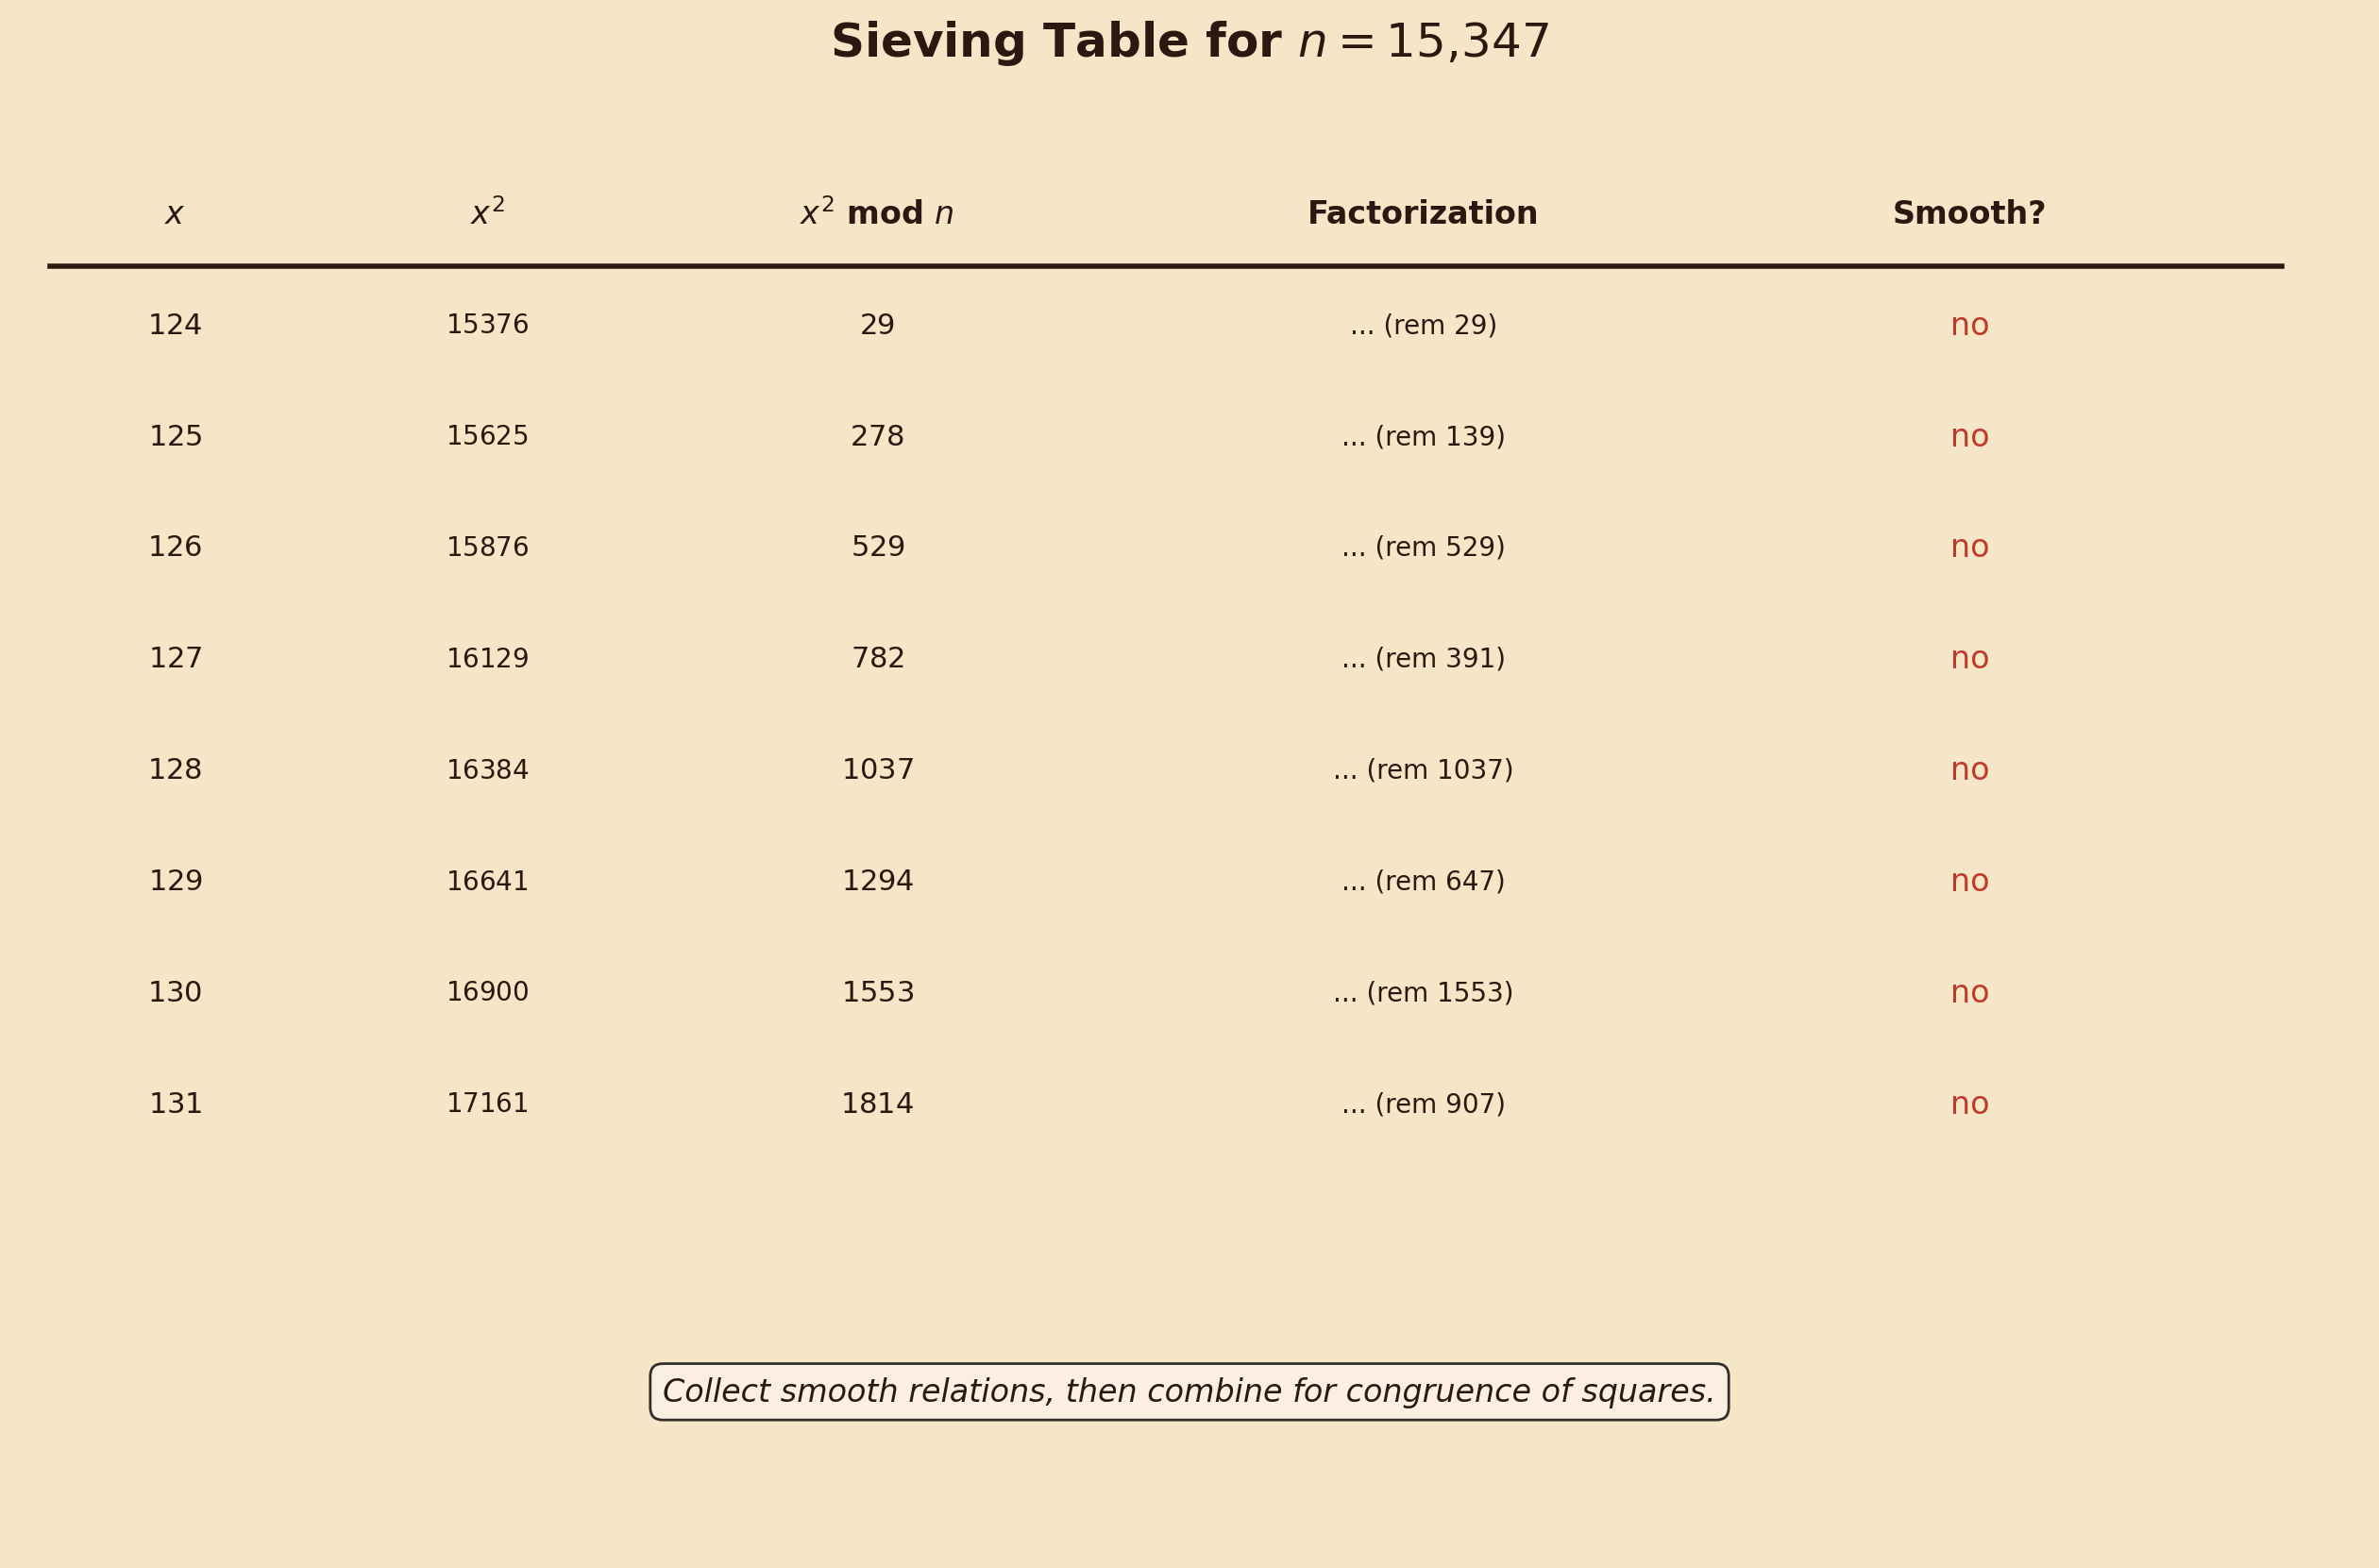
\includegraphics[width=0.85\textwidth]{Chapter11/images/fig13_sieving_table.png}
\caption{}
\end{figure}
A sieving table rendered as a large, elegant worksheet on parchment paper. Rows are indexed by \(x\) values. Columns show: \(x\), \(x^2\), \(x^2 \bmod n\), prime factorization of the residue, and a final column with either a green checkmark (smooth) or red cross (not smooth). The smooth rows glow faintly gold. At the bottom, the selected subset \(S = \{R_2, R_3, R_4, R_5\}\) is circled, with arrows leading to a final computation box showing \(\gcd(X - Y, n) = ?\).{]}


\begin{figure}[htbp]
\centering
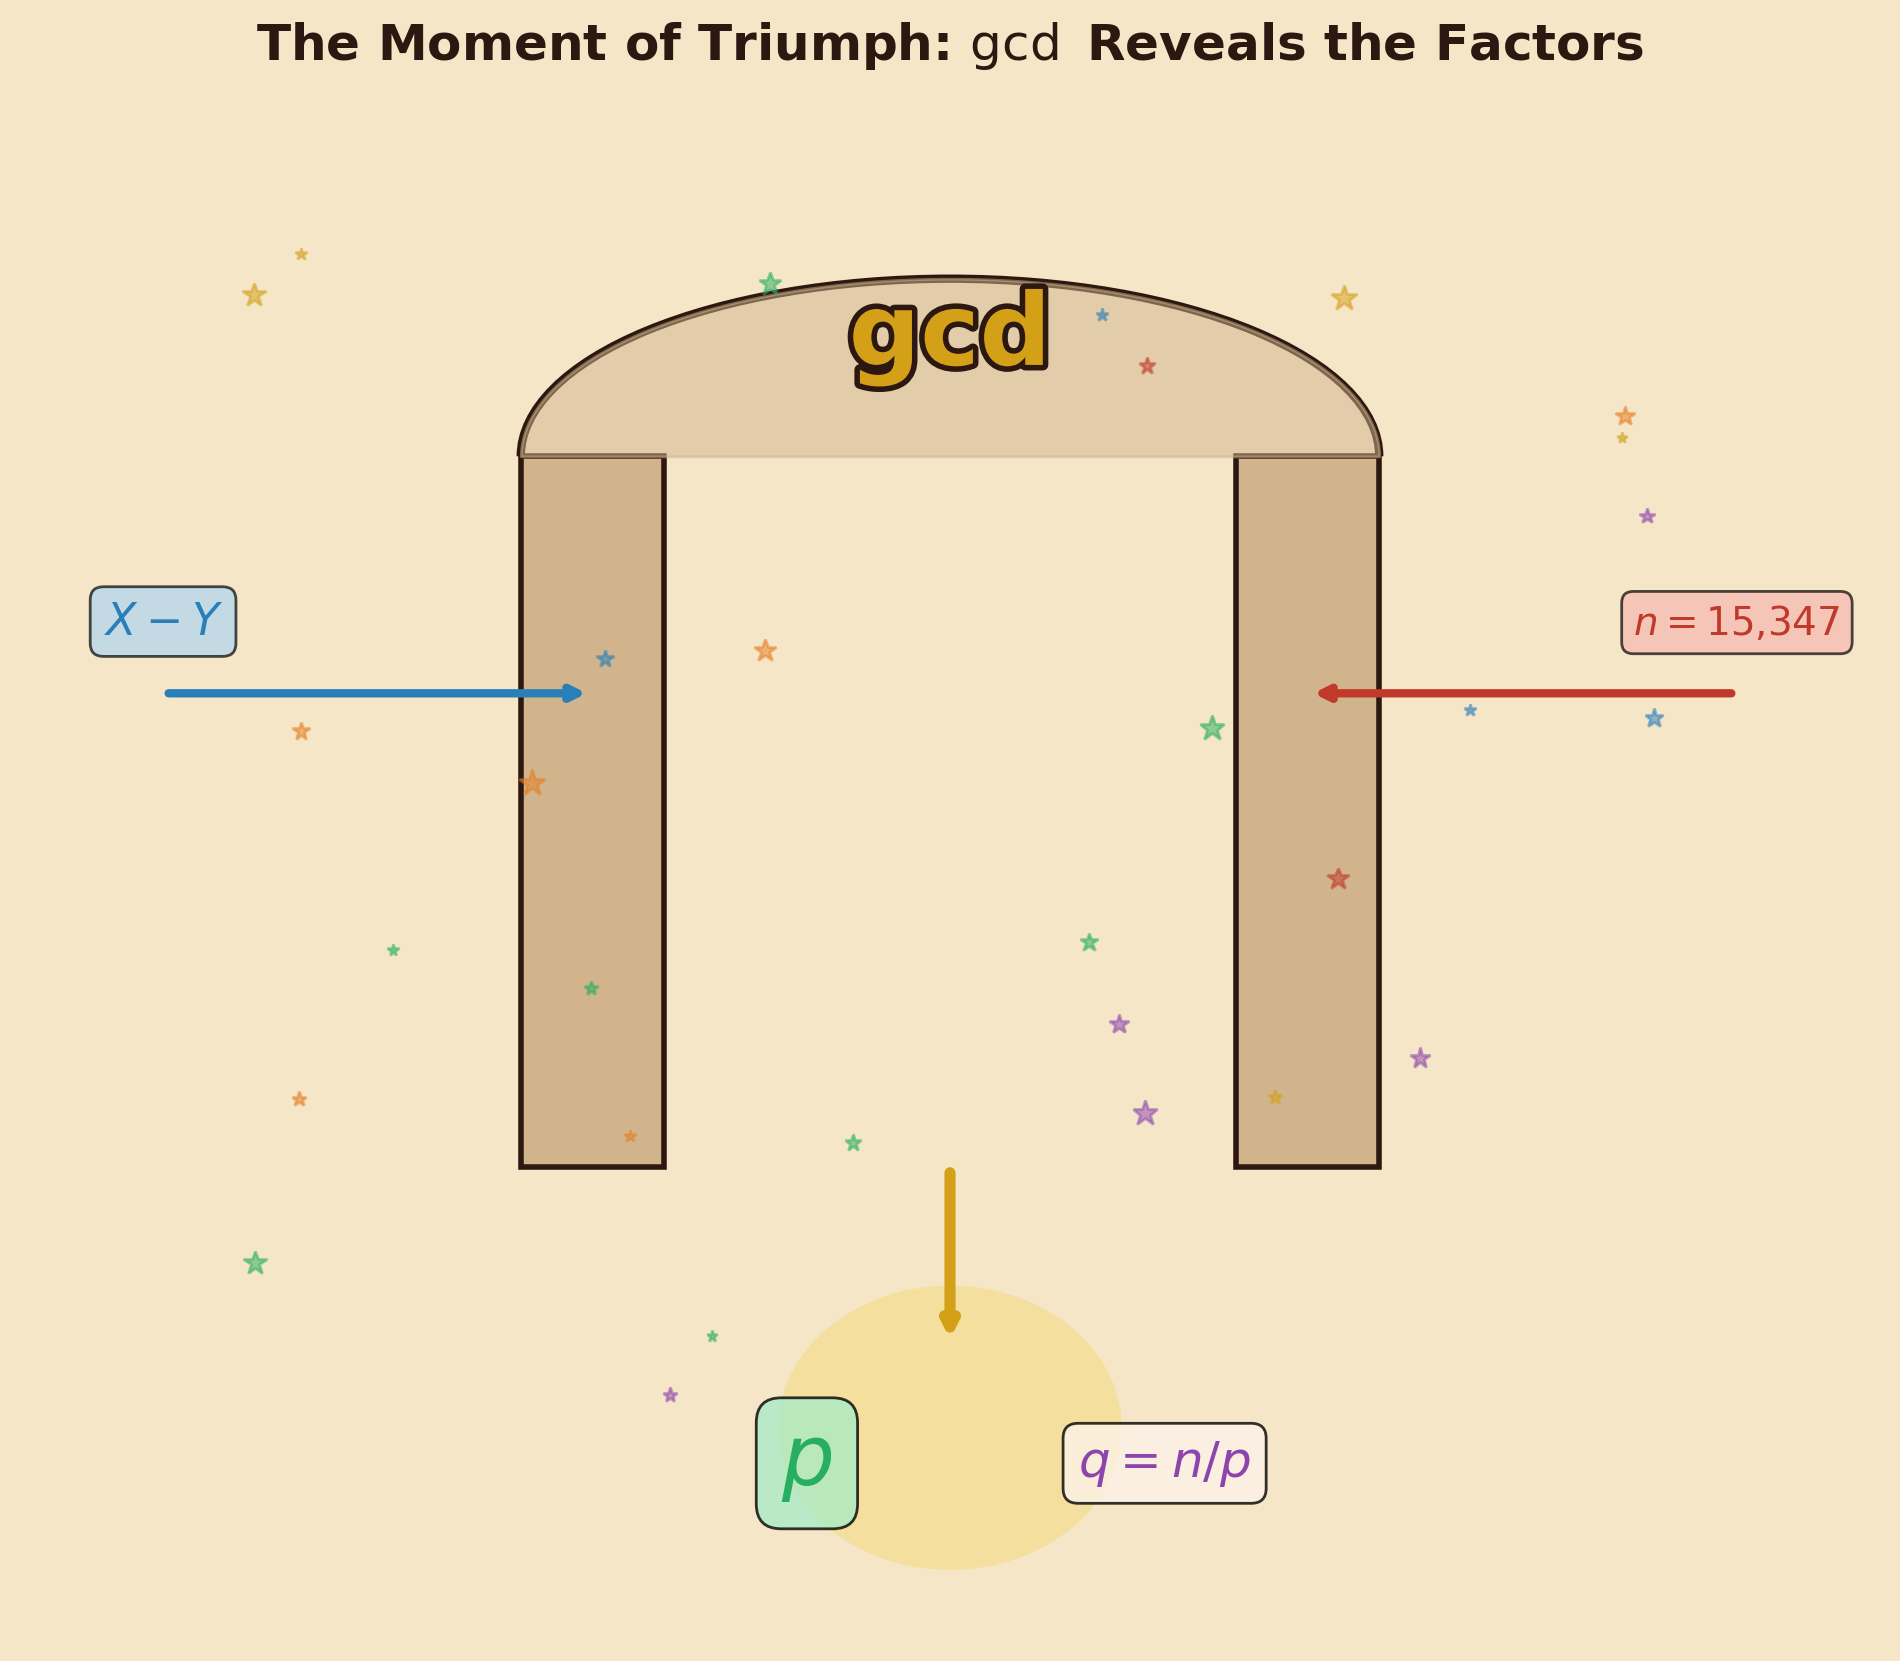
\includegraphics[width=0.85\textwidth]{Chapter11/images/fig14_gcd_gate.png}
\caption{}
\end{figure}
The final moment of triumph. A large ornamental ``\(\gcd\)'' gate --- like a classical archway --- stands at center. From the left, a banner reading ``\(X - Y\)'' feeds into the gate. From the right, a banner reading ``\(n = 15{,}347\)'' feeds in from the other side. Emerging from the bottom of the arch, bathed in a spotlight, stands a number: the factor \(p\). Beside it, in a slightly dimmer light, stands \(q = n/p\). Confetti falls. A small crowd of mathematicians in period dress applauds politely.{]}

\bigskip\noindent\rule{\linewidth}{0.4pt}\bigskip

\section{9. The Menagerie of Modern Sieves --- Dixon, QS, and NFS}
The congruence of squares is not a single algorithm. It is a \emph{philosophy} --- a way of thinking about factoring that has spawned an entire dynasty of ever-more-powerful methods, each one a new, cleverer incarnation of the same fundamental idea. It is as if mathematicians discovered a universal blueprint for a cathedral, and then spent forty years arguing about the best brand of bricks.

\textbf{Dixon's Random Squares (1981).} The simplest implementation of the philosophy. Choose a random integer \(x\) modulo \(n\). Compute \(x^2 \bmod n\). Check whether the result is \(B\)-smooth. If yes, record the relation. If no, try another \(x\). Repeat until you have \(k + 1\) smooth relations, then run Gaussian elimination over \(\mathbb{F}_2\) and extract the factor.

Dixon's method has the elegance of a haiku and the speed of a glacier. The probability that a random \(x^2 \bmod n\) is \(B\)-smooth is governed by Dickman's function, and for the optimal choice of \(B\), the total running time is \emph{subexponential} in \(\ln n\) --- faster than trial division, slower than polynomial time, occupying a curious middle kingdom of complexity:

\[L_n\!\left[\tfrac{1}{2}, \; \sqrt{2}\right] = e^{\sqrt{2} \cdot \sqrt{(\ln n)(\ln \ln n)}}.\]

This was a revelation in 1981: here was an algorithm that provably ran faster than any exponential-time method, yet relied on nothing more than random sampling and linear algebra.

\textbf{The Quadratic Sieve (QS, Pomerance, 1981).} Carl Pomerance's insight was to \emph{stop choosing \(x\) at random} and instead sieve a carefully chosen polynomial. Define \(f(t) = (t + \lceil \sqrt{n} \rceil)^2 - n\) for consecutive integer values of \(t\). Then \(f(t) \equiv (t + \lceil \sqrt{n} \rceil)^2 \pmod{n}\), so every \(B\)-smooth value of \(f(t)\) gives a smooth relation for free.

The genius of the QS is in how it \emph{finds} the smooth values. For each prime \(p\) in the factor base, the values of \(t\) where \(p \mid f(t)\) form an arithmetic progression with period \(p\) (or two progressions, one for each square root of \(n\) modulo \(p\)). So we can mark off --- \emph{sieve out} --- the multiples of each prime simultaneously, just as Eratosthenes sieved for primes two millennia ago. Only the values of \(t\) that survive being divided by enough small primes --- that is, the \(B\)-smooth values --- pass through the sieve. The running time improves to:

\[L_n\!\left[\tfrac{1}{2}, \; 1\right] = e^{\sqrt{(\ln n)(\ln \ln n)}},\]

roughly the square root of Dixon's time. The Quadratic Sieve was the fastest general-purpose factoring algorithm in the world from 1981 to approximately 1993.

\textbf{The Number Field Sieve (NFS, 1990s).} The reigning champion. Instead of sieving over the integers alone, the NFS sieves simultaneously over \(\mathbb{Z}\) and a carefully chosen \emph{number field} --- a ring of algebraic integers \(\mathbb{Z}[\alpha]\), where \(\alpha\) is a root of a polynomial selected to have small coefficients. The details are technical and deep, involving algebraic number theory, lattice reduction, and a two-stage sieve that collects ``algebraic'' and ``rational'' relations in tandem. The payoff is a running time of:

\[L_n\!\left[\tfrac{1}{3}, \; \left(\tfrac{64}{9}\right)^{\!1/3}\right] \approx e^{1.923 \cdot (\ln n)^{1/3} (\ln \ln n)^{2/3}}.\]

The exponent \(1/3\) (replacing the \(1/2\) of Dixon and QS) is the critical improvement: it means the NFS is asymptotically faster than the Quadratic Sieve for sufficiently large \(n\), and in practice the crossover occurs around \(100\) digits.

But --- and this is the point I want the reader to carry away from this section --- \emph{every single one of these algorithms, from the humblest to the mightiest, is executing the same playbook}. Find smooth relations. Build exponent vectors modulo \(2\). Find a linear dependency. Extract a congruence of squares. Compute a GCD. The Splitting Principle of Section 1 and the Guaranteed Dependency of Section 7 are the twin pillars on which the entire cathedral stands.

The factoring of RSA-768, a \(232\)-digit number, was completed in December 2009 by a team led by Thorsten Kleinjung. The computation required the equivalent of approximately \(2{,}000\) years of single-core processing time, distributed across hundreds of machines over a span of two and a half years. The sieving stage --- finding enough smooth relations --- consumed the vast majority of the time. The linear algebra stage --- Gaussian elimination over \(\mathbb{F}_2\) on a matrix with millions of rows and columns --- took several additional months on a supercomputer. And every cycle of computation, from first to last, rested on the theorem we stated in Section 1.


\begin{figure}[htbp]
\centering

\includegraphics[width=0.85\textwidth]{Chapter11/images/fig15_timeline.png}
\caption{}
\end{figure}
A horizontal timeline ribbon stretching from 1643 to the present, drawn in the style of a historical frieze. Milestone markers appear at: Fermat's method (1643) --- illustrated with a quill pen; Legendre's improvements (1798) --- a hand-cranked calculating machine; Morrison \& Brillhart's continued fraction method (1975) --- a room-sized mainframe with blinking lights; Dixon's random squares (1981) --- a dice being rolled; Pomerance's Quadratic Sieve (1981) --- a fine mesh sieve; Lenstra's Elliptic Curve Method (1987) --- a graceful elliptic curve, noted as ``a side branch: different ideas''; the Number Field Sieve (1993) --- an algebraic equation floating above a lattice; RSA-768 factored (2009) --- a massive supercomputer cluster with cables like tentacles. The ribbon is lightly colored in a gradient from sepia (past) to blue (present).{]}

\bigskip\noindent\rule{\linewidth}{0.4pt}\bigskip

\section{10. Philosophical Coda --- The Strange Democracy of Squares}
There is something philosophically arresting about the congruence of squares.

The fundamental theorem of arithmetic tells us that every integer greater than \(1\) has a \emph{unique} prime factorization. This uniqueness is the bedrock of number theory --- the reason we can speak of \emph{the} factors of \(n\) rather than \emph{some} factors. And yet this very uniqueness is fiendishly hard to \emph{discover}. Nature encodes every composite number with a unique fingerprint, then hides the fingerprint behind a computational wall that, for large enough numbers, exceeds the resources of every computer on Earth.

The congruence of squares says: don't try to find the factors directly. Instead, find two \emph{different representations} of the same residue as a square, and let the \emph{mismatch} between these representations betray the secret structure of \(n\). The method does not guess factors; it does not try to divide; it does not peek inside the number's construction. It simply observes that when two different square roots of the same value exist modulo \(n\), the number \(n\) has inadvertently revealed that it is not prime --- and the GCD operation extracts the confession.

What makes the sieve approach so powerful --- and so beautiful --- is the interplay of three distinct mathematical worlds:

\begin{enumerate}
\def\labelenumi{\arabic{enumi}.}
\item
  \textbf{Number theory} provides the stage: congruences, the GCD, the fundamental theorem of arithmetic, the distribution of primes.
\item
  \textbf{Combinatorics and probability} provide the search strategy: smooth numbers are rare but not too rare, and Dickman's function tells us exactly how long we must pan for gold before we find enough nuggets.
\item
  \textbf{Linear algebra} provides the endgame: the Guaranteed Dependency theorem transforms a pile of unrelated smooth relations into a single, decisive congruence of squares. The randomness of the search is transmuted into the certainty of algebra.
\end{enumerate}

The Guaranteed Dependency theorem deserves special emphasis in this regard. It is the fulcrum on which the entire enterprise balances. The search for smooth numbers is probabilistic --- we cannot predict which values of \(x\) will yield \(B\)-smooth residues --- but the theorem guarantees that \emph{once we have enough smooth relations, the rest is deterministic}. Gaussian elimination over \(\mathbb{F}_2\), a computation that takes seconds even when the matrix has millions of rows, will infallibly produce the dependency we need. The randomness is quarantined in the sieving phase; the algebra phase is as certain as sunrise.

And so we arrive at a curious democracy: every smooth number gets an equal vote. No single relation is more important than any other; it is only in \emph{combination} --- in the collective act of summing exponent vectors modulo \(2\) --- that they achieve the critical mass needed to factor \(n\). The sieve is not a duel between the cryptanalyst and the number; it is a ballot box, and the smooth numbers are the electorate. Once enough of them have voted, the outcome is decided.


\begin{figure}[htbp]
\centering
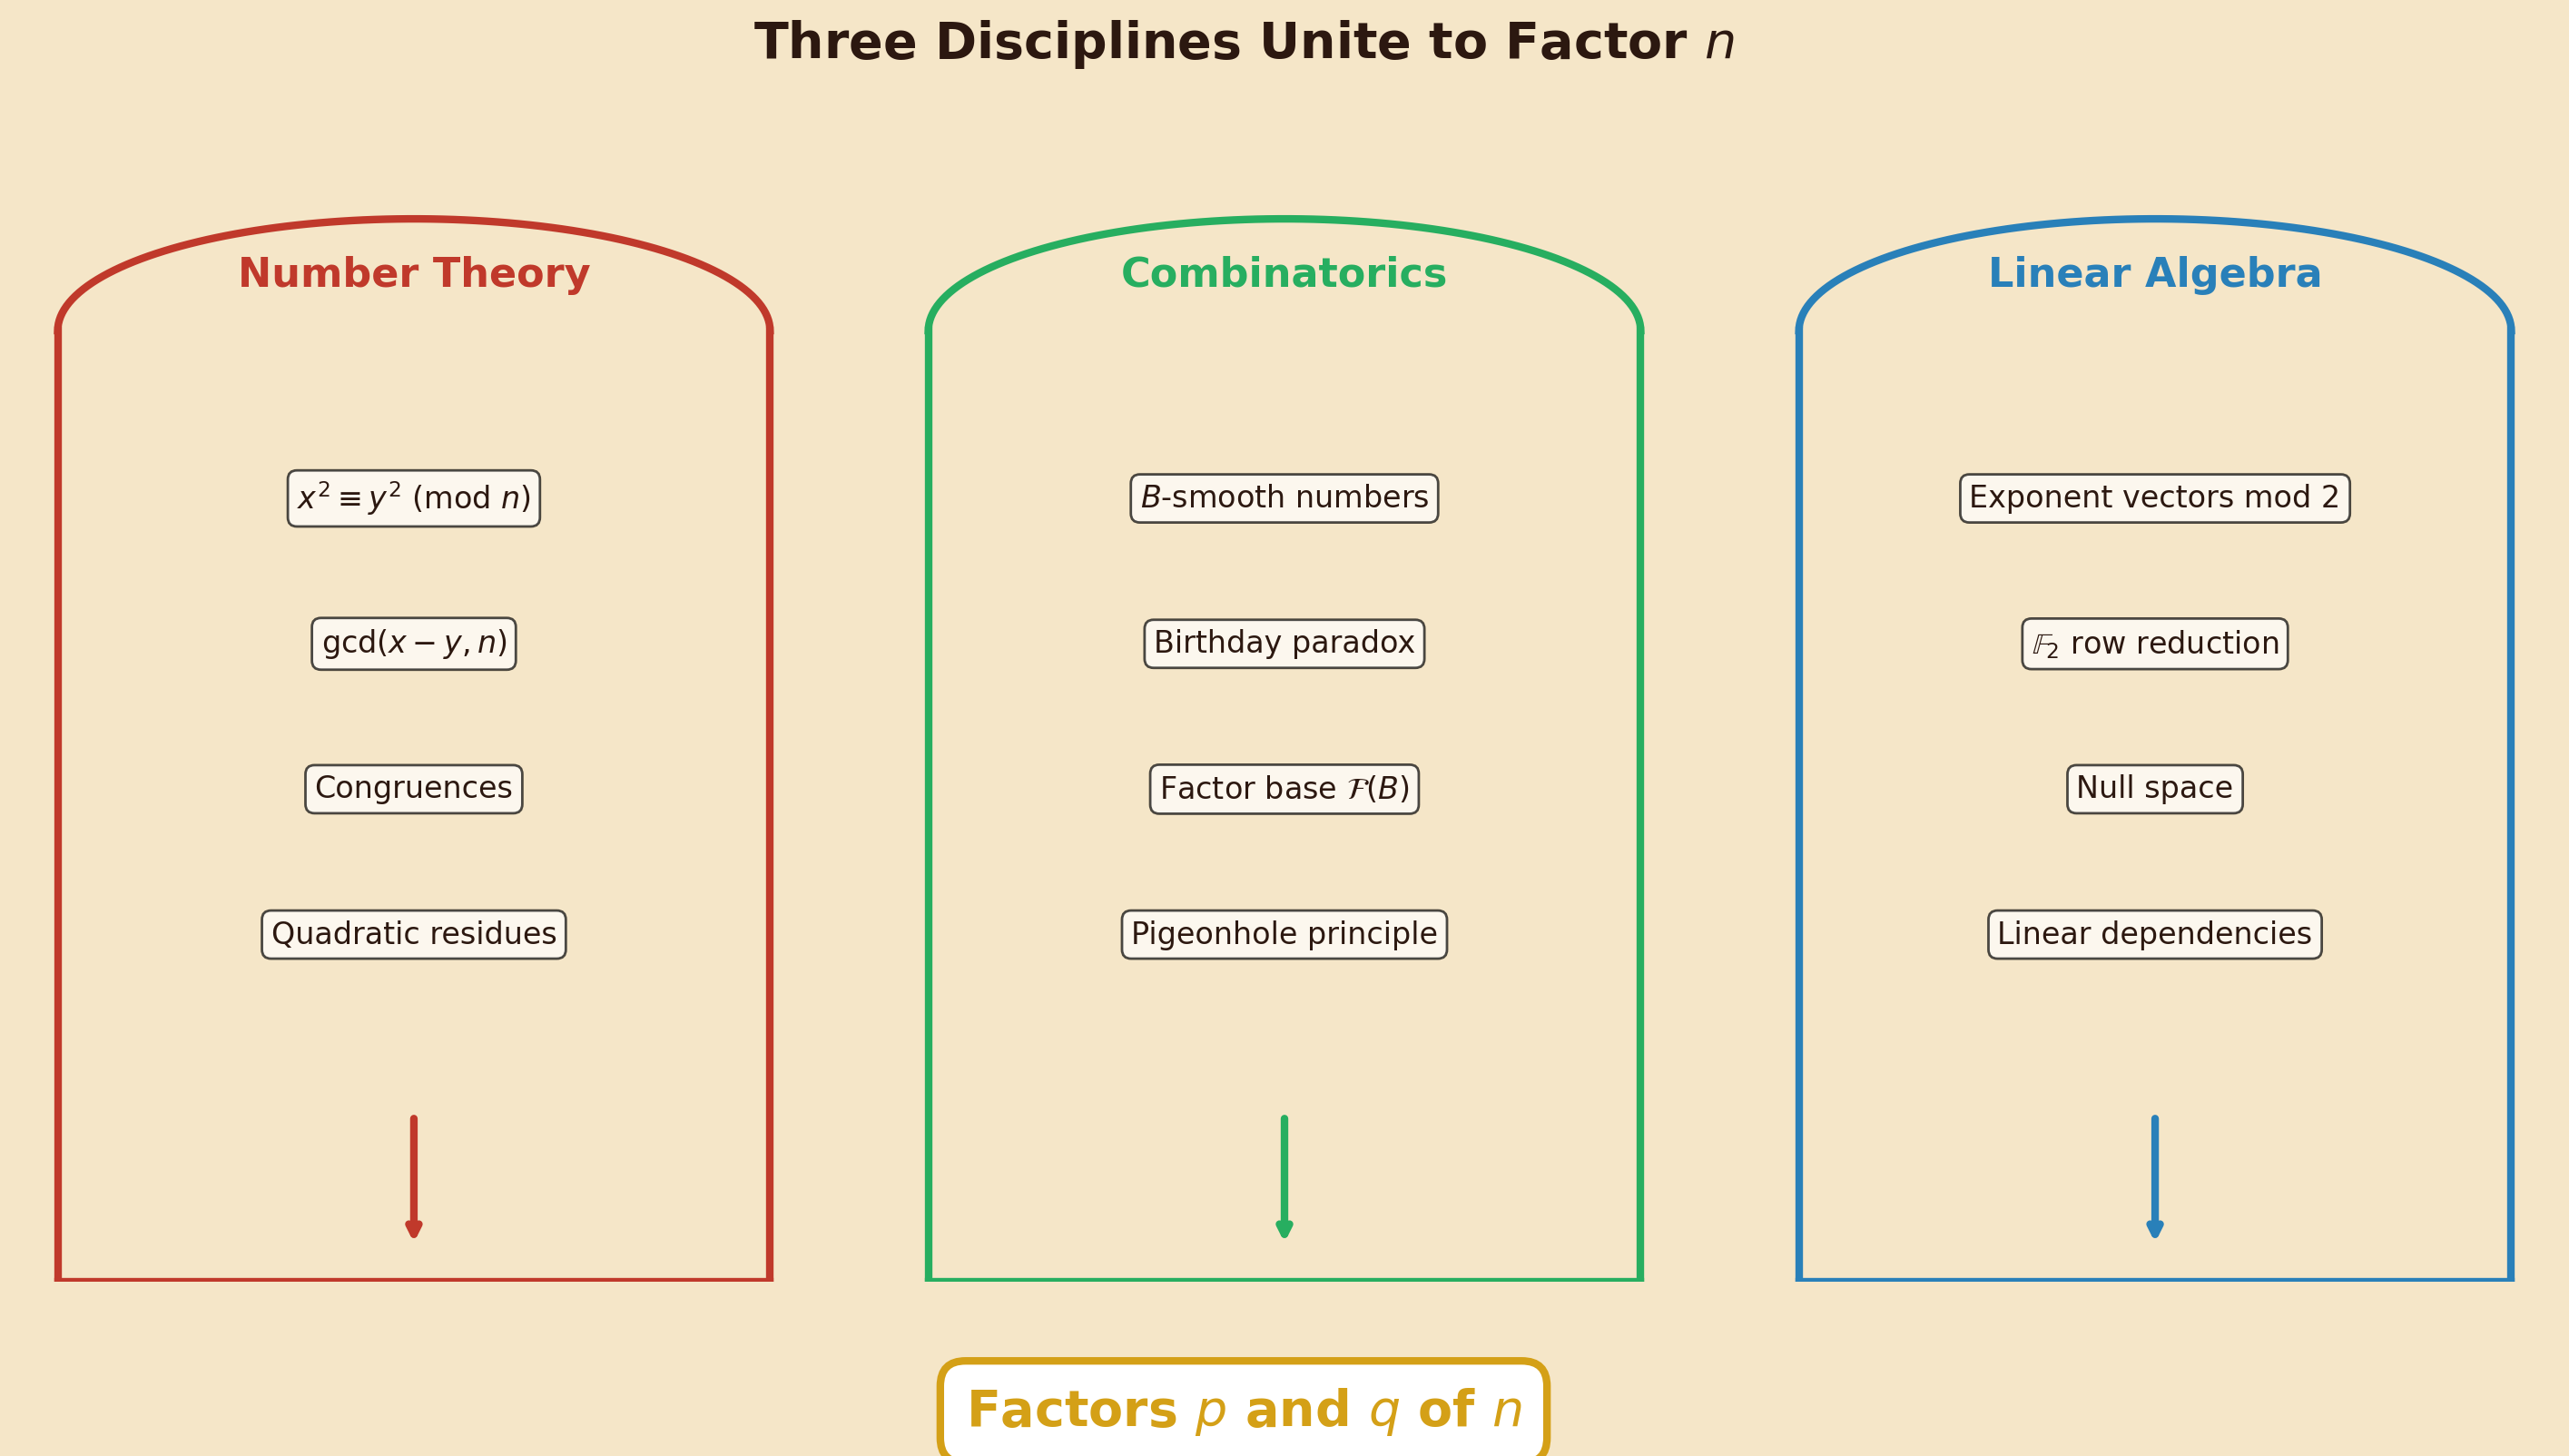
\includegraphics[width=0.85\textwidth]{Chapter11/images/fig16_triptych.png}
\caption{}
\end{figure}
A triptych panel, rendered in the style of a Renaissance altarpiece. The left panel shows a number theorist at a blackboard, chalking congruences and GCD computations; equations float in the air around her like mathematical halos. The center panel shows a combinatorialist tossing smooth numbers --- depicted as polished stones --- into labeled bins (one for each prime in the factor base), with a faint ``birthday paradox'' diagram visible on the wall behind him. The right panel shows a linear algebraist, spectacles perched on nose, performing row reduction on a vast matrix of \(0\)s and \(1\)s with a long pointer. All three panels converge at the bottom to a single glowing output: the factors \(p\) and \(q\) of \(n\), radiating golden light.{]}

One more remark before we close this chapter --- a forward-looking remark for readers who will join us in Chapters 12 and 13. The single GCD computation \(\gcd(x - y, n)\) that we have celebrated here is only the beginning. In the Quadruple Factor Theory of Chapter 12, we will see how moving from pairs \((x, y)\) to quadruples creates not one but \emph{several} independent factoring channels from a single algebraic relation. And in the GCD Cascade Factor Extraction of Chapter 13, the single GCD step generalizes to entire \emph{cascades} of GCD computations, each one extracting finer and finer information about the prime structure of \(n\). The Pythagorean tree and hyperbolic lattice methods we explored in earlier chapters --- the geometric roads from Chapters 3 and 4 --- offer yet another perspective: \emph{alternative sources} of smooth relations for the sieve, geometric roads to the same algebraic destination.

The congruence of squares, in other words, is not the end of the story. It is the beginning of a family of ideas, each one more powerful than the last, all sharing the same DNA. The magnificent sieve is not a single machine --- it is a \emph{species}, and evolution is far from over.

\bigskip\noindent\rule{\linewidth}{0.4pt}\bigskip

\emph{In the next chapter, we extend the Splitting Principle from pairs to quadruples, and discover that one equation can open not just two keyholes, but four.}
